\documentclass[a4,12pt]{article}
\usepackage[document]{ragged2e}
\usepackage[a4paper,left=2.54cm,right=2.54cm,bottom=3cm,top=3cm,text={18cm,20cm},footskip=32pt]{geometry}
\usepackage{latexsym} 	
\usepackage{amsmath}  
\usepackage{amsthm}	
\usepackage{amsopn}	
\usepackage{amscd}	
\usepackage{amssymb}
\usepackage{array}
\usepackage{actuarialsymbol}  
\usepackage{mathtools} 
\usepackage[utf8x]{inputenc} 
\usepackage{makeidx}  
\usepackage{multicol}  
\usepackage{multirow}
\usepackage{caption} 
\usepackage{float} 
\usepackage{enumerate} 
\usepackage{graphicx}   
\usepackage{subfig} 
\usepackage{booktabs} 
\usepackage{color}  
\usepackage[english]{babel} 
\usepackage{wasysym}
\usepackage{appendix} \usepackage{longtable}
\usepackage[authoryear]{natbib}
\usepackage[T1]{fontenc}
\usepackage{hyperref}
\usepackage{collref}
\usepackage{microtype}  \graphicspath{ {Figures/}} 
\usepackage{lmodern}
\usepackage{soul}
\usepackage{bm}
\usepackage{bookmark}
%    \usepgfplotslibrary{polar, fillbetween}
\usepackage{hyperref}
\usepackage{tikz}
\usepackage{authblk}
\usepackage{setspace}
\pagestyle{empty}

\makeatletter
\renewcommand{\@seccntformat}[1]{}
\makeatother

\doublespacing
    \usetikzlibrary{positioning, decorations.pathreplacing, arrows.meta, shapes}
%\usepackage{subcaption}



\begin{flushright} 
\raggedright
\textbf{Contribution Statement}

Although the Chinese ready-to-eat (RTE) food market has really taken off in the last decades, increasing its appeal towards researchers and practitioners, no study offers an attitudinal and behavioral analysis of the topic. Thus, some important features among consumers have not been recognized, as well as, the possible methodological frameworks to investigate it.
The present work is designed to be the first to profiling the typical consumer of RTE salads, studying a never explored market, and provide foresight to investors and policymakers. Second, we test competing models in order to reduce prediction errors; bringing new perspectives and findings to the literature of the fresh-cut; contributing to the nascent literature on using ML methods to predict customers' behaviors.


\end{flushright}.

\title{Chinese consumers’ attitude towards ready to eat salads by comparing traditional Logit with Machine Learning methods}

\author{}
%\author[1]{Hansstein Francesca}
%\author[2]{Nigri Andrea}
%\author[2]{Stasi Antonio}

%\affil[1]{\footnotesize{International Business School Suzhou, Xi'an Jiaotong-Liverpool University}}
%\affil[2]{Department of Agricultural sciences, Food, Natural resources and Engineering, University of Foggia}
\date{\today}

\begin{document}
	\maketitle
%\begin{abstract}
%\noindent
%\raggedright
%In the last decade, the ready to eat (RTE) food market has experienced substantial growth in China. The consumption of fresh-cut fruits and vegetables is a common eating trend for the expanding urban middle-class that is now more healthy-oriented than in the past. The attributes of RTE meals make it an attractive food choice for many consumers. However, to the authors’ knowledge, no study offers an attitudinal and behavioral analysis of the topic. Therefore, a survey among Chinese respondents was conducted to understand better the factors associated with RTE salad consumption.  The goal of this paper is thus twofold. First, we aim at profiling the typical consumer of RTE salads. Second, we test different machine learning classification algorithms on primary consumer data.
%Results show that consumption is more common among young respondents, females, healthy-oriented individuals at the beginning of their career. The role of the subjective norm is also positively associated with increased consumption of RTE salads. 
%\end{abstract}
%	\bigskip
	\begin{flushleft}
		\textbf{Keywords}: Ready to Eat Salads, Fresh-cut fruits \& vegetables, Chinese consumers, Machine Learning
	\end{flushleft}
%	\newpage
	



\section{Abstract}
In the last decade, the ready to eat (RTE) food market has experienced substantial growth in China. The consumption of fresh-cut fruits and vegetables is a common eating trend for the expanding urban middle-class that is now more healthy-oriented than in the past. The attributes of RTE meals make it an attractive food choice for many consumers. However, to the authors’ knowledge, no study offers an attitudinal and behavioral analysis of the topic. Therefore, a survey among Chinese respondents was conducted to understand better the factors associated with RTE salad consumption.  The goal of this paper is thus twofold. First, we aim at profiling the typical consumer of RTE salads. Second, we test different machine learning classification algorithms on primary consumer data.
Results show that consumption is more common among young respondents, females, healthy-oriented individuals at the beginning of their career. The role of the subjective norm is also positively associated with increased consumption of RTE salads. 
%--------------------------------------------------------------------------------------------
\section{Introduction}
\label{sec:1}
%--------------------------------------------------------------------------------------------

In recent years, the demand for ready-to-eat (hereafter RTE) food has increased noticeably in several world areas. According to current data\footnote{Fresh Food Packaging Market by Material (PE, PP, Paper, Aluminum, BOPET, PVC), Pack Type (Converted Roll Stock, Gusseted Bags, Flexible Paper, Corrugated Box), Application (Meat Products, Vegetables, Seafood, Fruits), and Region - Global Forecast to 2025, Markets and Markets, available at: \url{https://www.marketsandmarkets.com/Market-Reports/fresh-food-packaging-market-240678791.html}} , the growth of the fresh food packaging market is expected to go from USD 79.8 billion in 2020 to USD 95.2 billion in 2025, with a CAGR of 3.5\%. The Asia-Pacific Countries, including China, are leading this growth due to the rising demand for fresh foods, particularly vegetables and meat products, from the emerging middle-class.  RTE products include fresh-cut fruits and vegetables and other ready-to-eat meals like cereals, dairy, cold cuts, and meat. The nutritional benefits of RTE foods have been extensively acknowledged by experts \cite{Santeramo18}; \cite{Singla20}, although some others warn about the health risks associated with high sugar and fat content in some RTE foods \cite{Poti16}; \cite{Thike20}. Eating fruits and vegetables is associated with a robust immune system and risk reduction of many cardiovascular diseases and cancer \cite{Gibson12}; \cite{Gu21}. RTE fruits and vegetables are a practical way to increase their consumption as recommended by the health authorities of many countries. RTE meals can also provide a balanced diet in nutrient intake without giving up on taste and quality. This is also why they are often used in school menus \cite{Gibson19}. RTE salads are the most popular food among fresh food products, consisting of pre-cleaned leafy and fresh-cut mixed vegetables immediately ready for consumption or with few days of shelf-life. The consumption of pre-packaged salads is a well-established eating trend in many countries, and their popularity is exceptionally high among Western consumers.  The success of RTE fresh meals in Western countries has been interpreted as a sign of how innovation and integration between traditional agriculture and the food industry can meet the needs of modern consumers (\cite{Brennan13}; \cite{Massaglia19}). 
However, in other realities like China, the fresh food market is still expanding, and this circumstance offers an interesting investigation opportunity.  To the authors' knowledge, no one ever proposed an empirical study based on Chinese consumers' data, despite the preeminent growing expectations on the specific market. To cover this gap, the present study has a twofold goal. \\

Obj.1. By using survey data, the first objective of this study is to understanding socio-demographic, socio-economic, and psycho-social factors that affect the consumption of ready-to-eat salads among urban consumers.\\

Consumption patterns in urban China have dramatically changed in the last few years. Most consumers, especially young and urban, pay attention to their health, diet, and physical appearance much more than in the past, and this is reflected in their dietary choices. At the same time, most of them conduct a busy and fast-paced life, inspired by the need to enjoy life pleasures and save time and money. 
Moreover, as market research data show \cite{DaxueConsulting21}, health and future uncertainty have become more prominent preoccupations after the Covid-19 crisis. RTE fruits and vegetables are a consumption trend suitable to respond to these emerging consumer needs because do not require any time for preparation, are largely available, and offer a healthy meal substitution.  However, more research is needed to understand the driving forces that favor its consumption. In addition, the intake of vegetables in China is still below the level recommended by the Chinese dietary guidelines \cite{Xiao15} and the attributes of RTE salads, such as convenience and practicality, might help reach the expected consumption standard in the future. \\

Obj.2: The second objective of the paper is to apply an innovative methodological approach to consumer research. We propose a comparison among traditional Logit, random forests (RF), Deep Neural Network (DNN), Regression Tree (RT), and Support Vector Machine (SVM) in a food choice determinant analysis.\\

Consumers' behavior studies have most of the time referred to econometrics in order to predict choices (\cite{Storm19}). However, limited data associated with a high number of variables/factors have always been an issue to have easy interpretation and good prediction ability of models for the inference process. In recent years, however, different modelling approaches have been brought to light, also because of the remarkable increase in computational power \cite{Hastie16}. Machine learning (hereafter ML) approaches, in fact, could present advantages over traditional econometric models in certain situations. It is enormously useful in our context where a large number of factors may affect the fresh-cut customer's choice. Traditional techniques, such as the logistic regression, might be criticized because of rigid structure when compared to "distribution-free" approaches. However, they have the advantage of furnishing interpretability of coefficients, while the other approaches could be convenient for their ability to predict  (\cite{Lucun15}). To the best of our knowledge, there is a limited number of studies that use ML models for consumer profiling in relation to food choices. Summing up, the paper contributes to literature by offering manifold elements of innovation: \\
(i) studying a never explored market and provide foresights to investors and policy makers; (ii) testing competing models in order to reduce prediction errors; (iii) bringing new perspectives and findings to the literature of the fresh-cut; (iv) contributing to the nascent literature on using ML methods to predict customers' behaviors. 
The paper is structured as follows. Section 2 presents the research background. It discusses the literature review on RTE salads consumption and gives the policy and legal framework. Section 3 discusses the data and methods. Section 4 presents the results and Section 5 discusses the findings and Section 6 concludes. 


\section{Background}
\subsection{Literature review}
Literature presents plenty of evidence about food consumers' preferences towards fresh-cuts, even though mostly analyzing Western countries. In general, Europeans and US consumers are oriented towards quality, safety, nutritional elements, freshness, richness of assortment, etc. (\cite{Santeramo18}). In addition, other findings state that medium-high income consumer target, generally also high educated people (middle-class), is interested in purchasing products with a higher level of service and quality (\cite{Artes}; \cite{Watada19}, \cite{Soliva02}, \cite{Rico07}). However, common outcomes regard income as a driver of purchase (\cite{Marshall94}; \cite{Cassady07}) as well as time pressure, social environment and eating-out habits (\cite{Frewer13}; \cite{Buckley07}). Other papers highlight that quality, safety and labeled information are also important (\cite{Pilone17}; \cite{Santeramo18}; \cite{Pollard02};\cite{Baselice17}). All these contributions, however, present empirical evidence of Western countries. Among the countries of South East Asia that are most active in the development of fresh-cut products consumption, there is undoubtedly Thailand, whose model has been analyzed by FAO in its research (\cite{James10}, FAO 2010) 
Regarding fresh food products, the great majority of studies target Western consumers. All are empirical investigations aimed at segmenting the market and individualizing the perceived benefits and barriers. The literature indicates that consumption is prevalent among females, middle-income earners, and individuals below forty years old (\cite{Massaglia19}; \cite{Sgroi18}; \cite{VanLoo10}. In terms of time, money, and practicality, convenience is also an essential purchasing factor (\cite{Stiletto20}; \cite{Vidal13}. Other aspects that play a crucial role in the purchasing decisions are freshness (\cite{Dinnella14}), the understanding of food processing methods (\cite{Hicks09}; \cite{Liem16}), and the use of experience, visual intrinsic, and extrinsic attributes (\cite{Chonpracha20}; \cite{Pilone17}). Furthermore, food safety and shelf-life information are critical factors affecting RTE consumption (\cite{Baselice17}). 
Few studies target Asian consumers, and most of them do not focus on RTE fruits and vegetables precisely but also consider other types of food, like cereal-based meals.  A common finding among these studies is that the preferences and attitudes towards RTE food are strongly affected by experience and intrinsic attributes like freshness, odor, and taste (\cite{Kwon18}; \cite{Thienhirun18}). In Japan and South Korea, the market of fresh-cut products has been developed since the late 1990s. Fresh-cut meals are primarily used in schools and restaurants and also for personal consumption at home. Consumers in these regions perceived RTE products as safe and of high quality (\cite{Kim07}). Another study on Korean consumers found that consumption was higher among females, young, and healthy-oriented professionals. The only research targeting Chinese consumers investigated the demand for RTE imported meals. Results found that higher consumption of instant RTE foods is more frequent among commuters, and extrinsic attributes on food packages are often used as a cue to determine the product's quality (\cite{Lilavanichakul18}). Among these attributes, appearance is a fundamental purchasing driver when suggests freshness. This attribute is essential for Chinese consumers to determine food quality, especially the elderly (\cite{Hansstein17}).

\subsection{Policy and consumption framework}

Between 1960 and 2017, FAO statistics about food balance highlight that, while Western countries show decreasing consumption of fruits and vegetables, some Asian countries, including China, show the opposite. In fact, population growth, increasing trade, nutrition awareness, and migration are all factors having an incidence on those trends (\cite{FAO17}. In the last decades, the consumption of more nutritious foods increased worldwide, however, different trends have been observed For instance, fruit consumption rose in all areas, but vegetable consumption increased with different pace especially in Asian countries, as shown in Figure 1 (FAO, 2017). When correlating consumption and income, per capita fruit intake tends to rise with income, whereas vegetable consumption declines (\cite{FAO17}).

\begin{figure}[H]
		\centering
		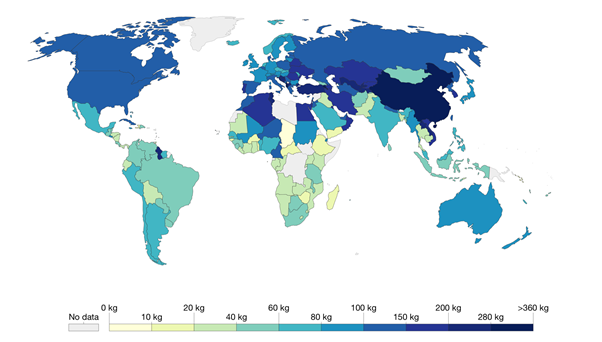
\includegraphics[width=.9\linewidth]{mondo}
		\caption{Map of evolving per capita consumption of vegetables (\cite{FAO17}).}
		\label{fig:mondo}
\end{figure}

Given the great concern about contemporary dietary habits, governments in several countries have launched informational and educational initiatives aimed at increasing public awareness about the benefits of F\&V. As a consequence, the effectiveness of these interventions have been evaluated by several authors(\cite{Seiders04}; \cite{Gordon06}; \cite{Mazzocchi09}). These studies lead to the development of guidelines and recommendations. Food policy and regulatory guidelines are prime tools to achieve a healthy diet in a population, with a remarkable impact on the health care systems and social and public health policies. 
China has also a long-standing commitment to policy guidance on food security-related nutrition. In the ’90s it launched the “China Nutrition Improvement Action Plan (1996-2000) \cite{HCAP}", followed by the "Management Measures for Nutrition Improvement (2010)” and the “National Nutrition Plan (2017–2030)”, which aims to improve nutrition and health on a national level and set national nutrition strategies for 2020 and 2030. Recently, China made great strides in food security and nutrition, implementing the "Healthy China Action Plan (2019–2030)" (HCAP). This regulation centralizes efforts to improve the populations’ nutrition status, facing many challenges, including obesity and chronic diseases.
 
Indeed, the fresh-cut sector - that includes RTE salads - plays a critical role in  the daily consumption of F&V, as recommended by the World Health Organization (\cite{WHO}). The “fresh-cut” sector offers convenience, in terms of time saving for washing and preparation, and freshness.. In line with the definition given by the International Fresh-Cut Produce Association (IFPA), fresh-cut F&V are minimally processed products that are washed, cut, mixed, and packed. Since their first appearance in Europe in the early 1980s, they have become more and more popular in consumers’ market baskets because of time convenience, quality and safety attributes that are generally valued positively by consumers (\cite{Artes}). RTE products are defined by the European Commission as  "food intended by the producer or the manufacturer for direct human consumption without the need for cooking or other processing to eliminate or reduce to acceptable level micro-organisms of concerns" (Regulation 2073/2005/EC). In China, RTE products regulation is included in the Food Safety Law of 2015 (HFG - Law and Intellectual Property, 2016). Given the risk of raw food contamination with dangerous bacteria, RTE food safety is currently the main concern for authorities. Therefore, encouraging proper handling and storage to avoid foodborne diseases is a priority for public and private food institutions.



%\hl{Descrizione ML}
%
%ML has advantages over traditional econometric models in certain situations.
%It is enormously useful in our context where a large number of factors may affect the fresh-cut customer's choice. Canonical inference tools, as in the case of logistic regression, may exhibit a rigid structure, leading to functional misspecification. On the contrary, the so-called "distribution-free" approaches do not impose a probabilistic assumption, therefore the functional relationship between variables is directly approximated from the data.
%Although some ML algorithms use hyperparameters, such as the number of trees and learning rates, these hyperparameters come by a fine-tuning procedure, thus are optimally chosen over a broad grid,
%Despite it is widely recognized that ML suffers from an interpretation issue, it fits our purpose of predicting the customer's behavior, particularly because the data are large and predictors are convoluted.
%Given the emergence of ML in prediction tasks for business, we expect the method to generate practical directions for our study. To the best of our knowledge, researchers have not explored ML models for food fresh-cut consumers' predictions.
%As a result, we apply random forests (RF) for predicting access to Chinese fresh-cut consumers' predictions, integrating the analysis with Deep Neural Network (DNN), Regression Tree (RT)... We selected these ML models over others because they scale with the volume of information without damaging statistical efficiency, are more versatile than others, and typically demonstrate good predictive accuracy as they are robust to outliers


%\hl{Conclusioni}

%The approach we follow is peculiar and new, providing manifold contributions. Indeed, (i) we bring new perspectives and findings of the fresh-cut products among Chinese customers, where the literature lacks a focus on this topic. (ii) Aiming at reducing the prediction errors, we contribute to the nascent literature on using ML methods to predict customers' behaviors.
%Thereby, this work aims at providing new insights to the analysis and prediction of fresh-cut customers' behavior in China even using recent innovations, offering peculiar information for both policymakers and practitioners.


%--------------------------------------------------------------------------------------------
\section{Models }
\label{sec:2}
%--------------------------------------------------------------------------------------------


\subsection{Logit}
To explore the role of specific factors affecting the consumption of ready-to-eat salads in China, we firstly run a logit model. Logit models are primarily used in discrete choice analysis and are helpful to assess the odds ratio of an outcome exposure or food choice. In consumer behavior and marketing research, logit models have been widely used to understand purchasing behavior (see for example \cite{Nevo11}; \cite{Roberts93}). 

Our independent variable can be treated as a realization of a random variable that follows a binomial distribution $Y_{i} \sim B\left(n_{i}, \pi_{i}\right)$.
Thus, we define generalized linear model with binomial response and link logit as:

\begin{equation}
\operatorname{logit}\left(\pi_{i}\right)=\mathbf{x}_{i}^{\prime} \boldsymbol{\beta}
\label{logit}
\end{equation}
where the logit of the underlying probability $\pi_{i}$ is a linear function of the predictors where $\mathbf{x}_{i}$ is a vector of covariates and $\boldsymbol{\beta}$ is a vector of regression coefficients. 
Thereby, $\beta_{j}$ represents the change in the logit of the probability associated with a unit change in the $j$ -th predictor holding all other predictors constant.
Exponentiating Equation \ref{logit} we find that the odds for the $i$ -th unit are given by 

\begin{equation} 
\frac{\pi_{i}}{1-\pi_{i}}=\exp \left\{\mathbf{x}_{i}^{\prime} \boldsymbol{\beta}\right\}
\end{equation} 
%This expression defines a multiplicative model for the odds. For example if we were to change the $j$ -th predictor by one unit while holding all other variables constant, we would multiply the odds by $\exp \left\{\beta_{j}\right\}$. To see this point suppose the linear predictor is $\mathbf{x}_{i}^{\prime} \boldsymbol{\beta}$ and we increase $x_{j}$ by one, to obtain $\mathbf{x}_{i}^{\prime} \boldsymbol{\beta}+\beta_{j}$. Exponentiating we get $\exp \left\{\mathbf{x}_{i}^{\prime} \boldsymbol{\beta}\right\}$ times $\exp \left\{\beta_{j}\right\}$. Thus, theexponentiated coefficient $\exp \left\{\beta_{j}\right\}$ represents an odds ratio. Translating the results into multiplicative effects on the odds, or odds ratios, is often helpful, because we can deal with a more familiar scale while retaining a relatively
The related log-likelihood function is defined as:
\begin{equation} 
\log L(\boldsymbol{\beta})=\sum\left\{y_{i} \log \left(\pi_{i}\right)+\left(n_{i}-y_{i}\right) \log \left(1-\pi_{i}\right)\right\},
\end{equation}
where $\pi_{i}$ depends on the covariates $\mathbf{x}_{i}$ and a vector of $p$ parameters $\boldsymbol{\beta}$ through the logit transformation of Equation \ref{logit} .

In our specification, the dependent variable indicated if the respondent regularly (at least three times per week) eats fresh-cut salads. The explanatory variables are age, income, seniority, household size, knowledge, fitness, source of information regarding RTE products, purchase location, and whether consumption occurs for snacking or for lunch.  The logit model was conducted on 70\% of the original sample as required by predictive statistics.  


\subsection{Machine Learning}


In this section, we deal with the wide framework of unsupervised learning which embraces various models such as Support Vector Machine, Neural Networks and Tree-based Models, used for both regression and classification problems.

According the statistical learning theory (SLT) the problem of supervised learning is formulated as follows. Given a set of training data $D=\left\{\left(\mathbf{x}_{1}, \mathrm{y}_{1}\right) \ldots\left(\mathbf{x}_{1}, \mathrm{y}_{1}\right)\right\}$ in $\mathrm{R}^{\mathrm{n}} \times \mathrm{R}$ sampled according to unknown probability distribution $\mathrm{P}(\mathbf{x}, \mathrm{y}),$ and a loss function $\mathrm{L}(\mathrm{y}, \mathrm{f}(\mathbf{x}))$ that measures the error done when, for a given $\mathbf{x}, \mathrm{f}(\mathbf{x})$ is "predicted" instead of the actual value $y$.

It is worth pointing out that there is no information on the underlying joint probability functions. Therefore, it is necessary to perform a "distribution-free" approach, where the only information available is a training dataset.

The problem consists in finding a function $f$ that minimizes the expectation of the error on new data, that is, find a function $\mathrm{f}$ that minimizes the expected error:
$$
\int \mathrm{L}(\mathrm{y}, \mathrm{f}(\mathbf{x})) \mathrm{P}(\mathbf{x}, \mathrm{y}) \mathrm{d} \mathbf{x} \mathrm{dy}
$$
Since $\mathrm{P}(\mathbf{x}, \mathrm{y})$ in unknown, we need to use some induction principle in order to infer from the 1 available training examples a function that minimizes the expected error. The principle used is Empirical Risk Minimization (ERM) over a set of possible functions, called hypothesis space. Formally this can be written as minimizing the empirical error:
$$
\frac{1}{l} \sum_{\mathrm{i}=1}^{l} \mathrm{~L}\left(\mathrm{y}_{\mathrm{i}}, \mathrm{f}\left(\mathbf{x}_{\mathrm{i}}\right)\right)
$$
%with $\mathrm{f}$ being restricted to be in a space of functions - hypothesis space - say $\mathrm{H}$. 

Machine Learning tools are the so-called “nonparametric” models. “Nonparametric” does not mean that the ML models do not have parameters at all. On the contrary, their “learning” is the crucial issue here, indeed, unlike in classic statistical inference, the parameters are not predefined and their number depends on the training data used. 


\subsection{DNN}

The term NN refers to a mathematical model inspired by the human brain. It allows computational models composed of multiple processing layers to learn representations of data characterized by multiple levels of abstraction, solving even the most complex problems. Its architecture includes neurons, synaptic connections that link the neurons, and learning algorithms (backpropagation). NN works as a weighted regression in which each unit gets “weighted” information through synaptic links from the other connected ones, returning an output by using an activation function that transforms the weighted sum of input signals. Albeit DL embodies a broad variety of networks differing from each other by the architectural structure, in this section the basic scheme of NN has been presented, the so-called feedforward structure.
NN training involves an unconstrained optimization problem where the aim is to minimize a
function in high dimensional space, the so-called loss function, that measures the difference between the predicted values and observed ones.
The back-propagation is the most used algorithm for the training of NNs. The algorithm compares the predicted values against the desired ones (objective)
and modifies the synaptic weights by back-propagating the gradient of the loss function. Schematically,
the procedure alternates forward and backward propagation steps:
\begin{itemize}
\item in the forward step, the prediction is computed fixing the synaptic weights,
\item in the backward step, the weights are adjusted in order to reduce the error of the network.
\end{itemize}
The NN iteratively performs forward and backward propagation and modifies the weights to
find the combination that minimizes the loss function $\mathcal{L}$.

\subsection{SVM}

Support Vector Machines originated as an altertinative to Neural Networks in the wide context of statistical learning, offering a solution to this trade-off by arbitrarily fixing model accuracy and minimising model complexity; in this way it is able to manage overfiting.\\ 
In a classification problem, this translates into an optimal solution identified by a linear hyperplane which correctly classifies observed data and lies as far as possible from them.\\


\subsection{Random Forest}
Since Regression Trees usually produces low bias and high variance estimations, they became a good candidate for ensemble methods. 
Indeed, Random forests basically consist in building an ensemble of decision trees grown from a randomized variant of the tree, this method is useful to get the error reduction pulling down the prediction variance, preserving the bias
Starting from a single learning set,  the basic idea is to introduce a random perturbation into the learning procedure in order to introduce a differentiation among the trees and combine the predictions of all these trees using aggregation techniques. 
\cite{Breiman96} proposed a first aggregation method the so-called bagging in which the different trees, are built by using random bootstrap copies of the original data. 
Its natural evolution, the random forests, was developed by the same author in 2001 \cite{Breiman01}. 
In the random forests the bagging approach has been extended and combined with randomization of the input variables that are used when considering candidate variables to split internal nodes $t$. 
In particular, instead of looking for the best split $s^*$ among all variables, the algorithm chooses a random subset of $K$ variables for each node and then determines the best split using these variables. \\

\subsection{Performance assessment Cross-validation}
In a $k$ -fold cross-validation $(C V)$, the original dataset is randomly partitioned into $k$ subsets of approximately equal sizes. At each of the $k$ CV iterations, one of the folds is chosen as the test set, while the $k-1$ others are used for training. The considered performance measure is computed based on the test set. After the $k$ iterations, the performances are finally averaged over the iterations. In our study, we perform 10 repetitions of stratified 5 -fold $\mathrm{CV}$, as commonly recommended (\cite{Bischl12}) . In the stratified version of the CV, the folds are chosen such that the class frequencies are approximately the same in all folds. The stratified version is chosen mainly to avoid problems with strongly imbalanced datasets occurring when all observations of a rare class are included in the same fold. By $" 10$ repetitions", we mean that the whole CV procedure is repeated for 10 random partitions into $k$ folds with the aim to provide more stable estimates.


\subsection{Accuracy Prediction}
For binary target variables, we evaluate the level of accuracy and its $95 \%$ confidence interval (CI), true positive rate (Sensitivity), true negative rate (Specificity), and Cohen's Kappa (\cite{Cohen60}). We define  $y=1$ for a regular consuption of RTE and 0 otherwise. Then a $2 \times 2$ confusion matrix has elements $a_{\text {row,column }}$ with predicted conditions $\widehat{y}=\{1,0\}$ on rows and true conditions $y=\{1,0\}$ on columns. The statistics are defined by,
\begin{equation}
\text {Accuracy }=\frac{a_{11}+a_{22}}{a_{11}+a_{12}+a_{21}+a_{22}}\\
\end{equation}

\begin{equation}
\begin{array}{l}
\text {Sensitivity or True Positive Rate (TPR)} =\frac{a_{11}}{a_{11}+a_{12}}\\
\\
\text {Specificity or True Negative Rate (TNR)} =\frac{a_{22}}{a_{21}+a_{22}}
\end{array}{}
\end{equation}
\\
We calculate accuracy that refers to the portion of customers correctly classified with respect to RTE regular consumption.
We calculate the 95\% confidence interval using accuracy’s standard deviation generated through iterations. 
Sensitivity refers to the proportion of regular RTE consumers correctly identified as such. Poor sensitivity implies a large number of inclusion errors, i.e. identifying RTE consumers when in fact they are not.  Specificity refers to the proportion of customers correctly predicted to be occasional RTE consumers. Poor specificity implies a large number of exclusion errors. Cohen's Kappa statistic measures the agreement for categorical variable relative to what would be expected by chance. That is,

\begin{equation}
\begin{array}{l}
\text{Kappa}=1-\frac{1-\text { Accuracy }}{1-\mathrm{EP}} \\
\\
\text{EP}=\frac{\left(a_{11}+a_{12}\right)\left(a_{11}+a_{21}\right)+\left(a_{21}+a_{22}\right)\left(a_{12}+a_{22}\right)}{\left(a_{11}+a_{12}+a_{21}+a_{22}\right)^{2}}
\end{array}
\end{equation}


where, accuracy of prediction is the observed probability, and $E P$ is the probability of random agreement or expected probability. Cohen's Kappa becomes zero if there is no agreement among the predicted and observed response other than what would be expected by chance. The reported output also provides the McNemar test and the numerical and graphical representation of the ROC curve and the relative area under the curve (AUC) values \footnote{The area under the (ROC) curve, summarizes the classifier performance. The larger area under the curve the better the classifier.}.

%--------------------------------------------------------------------------------------------
\section{Empirical Analisys }
\label{sec:3}
%--------------------------------------------------------------------------------------------

\subsection{Data} 
The cross-sectional study examined the consumption of ready-to-eat salads among a sample of Chinese consumers. The consumption of prepackaged fruits and vegetables has increased in China in the last years, especially among young urban workers. Fresh salads are a versatile, healthy, and convenient meal that can easily substitute or accompany a lunch, a snack, or a dinner. A total of 524 questionnaires were collected by trained interviewers between January and March 2019, in the area of Suzhou and Shanghai. The study employed a convenient sample, and participants took part in the survey voluntarily.  The questionnaire was part of a larger project that collected information on ready-to-eat fruits and vegetables. It was designed following the literature on the consumption of fruits and vegetables and included several sections. Questions included in the analysis are available in the Appendix (\ref{App.Q}). The project's coordinators built the first version in English, and the questionnaire was later translated into Chinese by a bilingual speaker. Researchers conducted a questionnaire validation through a pilot test on a smaller sample of potential respondents to make sure that Chinese speakers correctly understood all the questions.  The core analysis included behavioral questions on consumption of ready-to-eat-salads, socio-demographic variables, knowledge of fresh-cut products, subjective norms, and other questions on respondents' habits. All variables included in the model were categorical. Data were analyzed by the authors and are now currently stored on a private cloud owned by the authors.

\paragraph{Variable transformation} 
Most variables did not require any modification, with the exception of two indicators that were built after data collection. The first indicator is "knowledge," a variable measuring respondent's level of awareness towards packaged ready-to-eat fruits and vegetables compared with their regular alternative. Respondents had to indicate whether six statements were true or false. They were: "RTE products must be washed before being consumed," "RTE products are more treated," "RTE products are healthier," "RTE products are industrial products," and "RTE products are more controlled and selected."  If the respondent answered correctly, the variable value was 1, and 0 otherwise. We then built the variable "knowledge" so that each respondent could obtain a score ranging from 0 to 6. Knowledge was categorized as low if the score was below 2, medium if between 2 and 4, and high if above or equal to 5. 
The second variable that needed recoding was "subjective norm."  Respondents were asked to indicate how important was the opinion towards fresh-cut products of their relevant people. Specifically, we included questions about family, friends, colleagues, and social media influencers. Following the statistical procedure indicated in \cite{Acock08}, we built the indicator "subjective norm" using the mean score method.  
Principal component analysis and alpha Cronbach were determined before calculating the scores. The subjective norm's eigenvalue was unique with a value of 2.18, and the Alpha Cronbach's between the four items was 0.71. The eigenvalue of knowledge was 1.95, and the correlation between items 0.60. 

Table \ref{table:statistics} reports the descriptive statistics of the whole sample. There is a slight prevalence of female respondents, and, overall, 57\% of participants have less than 30 years old. The presence of young people in the sample is also reflected by the distribution of job seniority level, with only 15\% of respondents occupying managerial roles. Income distribution is even among the four ranges of the variable. One-fourth of respondents regularly consume RTE salads. As specified in the question, regular consumption indicated that respondents purchase an RTE salad about three times per week. Consumption is mainly for snacking (60\%) or for lunch (60\%). Purchasing locations are the supermarket (75\%) and convenience stores (25\%). About half of respondents regularly practice some physical activity during their free time (48\%). About 10\% of respondents exhibit a low level of subjective norm, meaning they give little importance to others' opinion in their behavioral choices. About 52\% and 37\% have instead medium and high subjective norm's levels. 

\begin{table}[H]
\center
\begin{tabular}{l|l|l|l}
\hline
\textbf{Variable}                 & \textbf{Frequency} & \textbf{Variable}                              & \textbf{Frequency} \\ \hline
\textbf{Gender}                   & \textit{}          & \textbf{Regular consumption of RTE}            & \textit{}          \\ \hline
\textit{Female}                   & \textit{52\%}      & salads                                         & \textit{}          \\ \hline
\textit{Male}                     & \textit{48\%}      & \textit{Yes}                                   & \textit{25\%}      \\ \hline
\textbf{Age}                      & \textit{}          & \textit{No}                                    & \textit{75\%}      \\ \hline
\textit{21-25}                    & \textit{23\%}      & \textbf{Fitness}                               & \textit{}          \\ \hline
\textit{26-30}                    & \textit{34\%}      & \textit{Yes}                                   & \textit{48\%}      \\ \hline
\textit{31-35}                    & \textit{12\%}      & \textit{No}                                    & \textit{52\%}      \\ \hline
\textit{36-40}                    & \textit{17\%}      & \textbf{Learning-advertising}        &                    \\ \hline
\textit{\textgreater{}40}         & \textit{14\%}      & \textit{Yes}                                   & \textit{76\%}      \\ \hline
\textbf{Income}                   & \textit{}          & \textit{No}                                    & \textit{24\%}      \\ \hline
\textit{Below 15,000rmb}          & \textit{28\%}      & \textbf{Learning-social media}       &                    \\ \hline
\textit{Between 15 and 20,000rmb} & \textit{25\%}      & \textit{Yes}                                   & \textit{31\%}      \\ \hline
\textit{Between 20 and 25,000rmb} & \textit{21\%}      & \textit{No}                                    & \textit{69\%}      \\ \hline
\textit{More than 25,000rmb}      & \textit{27\%}      & \textbf{Purchasing-supermarket}       & \textit{}          \\ \hline
\textbf{Job seniority level}      & \textit{}          & \textit{Yes}                                   & \textit{75\%}      \\ \hline
\textit{Entry}                    & \textit{40\%}      & \textit{No}                                    & \textit{25\%}      \\ \hline
\textit{Middle}                   & \textit{45\%}      & \textbf{Purchasing-convenience store} & \textit{}          \\ \hline
\textit{Managerial}               & \textit{15\%}      & \textit{Yes}                                   & \textit{49\%}      \\ \hline
\textbf{Household size}           & \textit{}          & \textit{No}                                    & \textit{51\%}      \\ \hline
\textit{One or two people}        & \textit{18\%}      & \textbf{Consumption for snacking}              & \textit{}          \\ \hline
\textit{Three people}             & \textit{50\%}      & \textit{Yes}                                   & \textit{60\%}      \\ \hline
\textit{More than three people}   & \textit{32\%}      & \textit{No}                                    & \textit{40\%}      \\ \hline
\textbf{Knowledge of RTE}         & \textit{}          & \textbf{Consumption for lunch}                 & \textit{}          \\ \hline
\textit{Low}                      & \textit{25\%}      & \textit{Yes}                                   & \textit{60\%}      \\ \hline
\textit{Medium}                   & \textit{39\%}      & \textit{No}                                    & \textit{40\%}      \\ \hline
\textit{High}                     & \textit{36\%}      &                                                & \textit{}          \\ \hline

\textbf{Subjective norm}         & \textit{}          & \textbf{}                 & \textit{}          \\ \hline
\textit{Low}                      & \textit{10.79\%}      & \textit{}                                   & \textit{60\%}      \\ \hline
\textit{Medium}                   & \textit{51.76\%}      & \textit{}                                    & \textit{40\%}      \\ \hline
\textit{High}                     & \textit{37.44\%}      &                                                & \textit{}          \\ \hline
    
\end{tabular}
\caption{Descriptive Statistics}
\label{table:statistics}
\end{table}

\\

\begin{table}
\begin{center}
\begin{tabular}{lcll }
\hline
& & $\beta_j$ & s.e. \\
\hline
(Intercept)  &            & $-3.63^{***}$  & $(0.99)$    \\  
\hline
\textbf{Gender (F)}       &        & $-1.04^{**}$   & $(0.39)$      \\
\hline
\multirow{ 2}{*}{\textbf{Age (21-25)}}
 & 26-30  &                 $1.32^{*}$       & $(0.58)$      \\
 & 31-35                  & $0.44$              & $(0.64)$      \\
 & 36-40                  & $0.35$              & $(0.58)$      \\
 & >40                & $-0.76$             & $(0.72)$      \\
\hline
\multirow{ 2}{*}{\textbf{Income (Inc. <15k )}}
 & 15k< Inc. \le20k                 & $-1.61^{**}$  & $(0.53)$      \\
 & 20k< Inc. \le25k                & $-1.12$           & $(0.58)$      \\
 & Inc. >25k                & $-0.38$          & $(0.49)$      \\
\hline
\multirow{ 2}{*}{\textbf{Job Seniority (Entry)}}
&Middle               & $1.61^{***}$   & $(0.45)$      \\
&Managerial            & $0.91$               & $(0.64)$      \\
\hline
\multirow{ 2}{*}{\textbf{Household size (1-2 people)}}
& 3 people          & $0.20$            & $(0.57)$      \\
&>3 people           & $1.17^{*}$      & $(0.59)$      \\
\hline
\multirow{ 2}{*}{\textbf{Knowledge (Low)}}
&Medium             & $0.10$          & $(0.44)$      \\
&High           & $-0.31$        & $(0.50)$      \\
\hline
\textbf{Fitness (No)}           &      & $1.39^{***}$    & $(0.38)$      \\
\hline
\multirow{ 2}{*}{\textbf{Learning}}
&Advertising (0-1)        & $-1.18^{**}$     & $(0.42)$      \\
&Social (0-1)     & $-1.05^{*}$     & $(0.42)$      \\
\hline
\multirow{ 2}{*}{\textbf{Purchasing}} 
&Supermarket (0-1)        & $1.04$            & $(0.56)$      \\
&Conv. store (0-1)    & $0.51$        & $(0.42)$      \\
\hline
\multirow{ 2}{*}{\textbf{Consumption}} 
&Lunch (0-1)   & $0.61$        & $(0.38)$      \\
&Snacking (0-1)   & $-0.84^{*}$          & $(0.41)$      \\
\hline
\multirow{ 2}{*}{\textbf{Subjective norm (Low)}} 
& Medium   & $0.42$                  & $(0.70)$     \\
& High   & $1.52^{*}$            & $(0.76)$     \\
\hline

AIC                      & & $284.67$      \\
BIC                      & & $372.58$      \\
Log Likelihood       &     & $-118.33$     \\
Deviance              &    & $236.67$      \\
\hline
\multicolumn{2}{l}{\scriptsize{$^{***}p<0.001$; $^{**}p<0.01$; $^{*}p<0.05$}}
\end{tabular}
\caption{Logit model estimation}
\label{table:coefficients}
\end{center}
\end{table}

Table \ref{table:coefficients} reports the logit regression results performed on the 70\% of the overall sample.  The table reports the coefficients, standard errors, and significance level. Concerning socio-demographic results, we observed that male respondents are less likely to regularly consume RTE salads compared to female respondents (p < 0.000). Respondents between 26 and 30 years old were more likely to consume RTE salads than younger respondents (p < 0.05). A lower income was also significantly associated with the consumption of fresh salads. A similar result was observed for respondents in a middle-level job compared to those at the entry-level. 
Regarding the other variables, we observed that fitness and subjective norm were positively associated with RTE salad consumption. Social and advertising did not seem to be the main channels through which consumers find information about fresh-cut products. Frequent consumers were more likely to consume RTE salads for lunch and buy them at the supermarket. 
These results, altogether, are helpful to outline the profile of the typical Chinese consumer of RTE salads. Young, prevalently females, at middle-career level, healthy oriented, pragmatic, and inclined to listen to his/her group reference opinions for food purchasing. 

\subsection{Prediction}
In this section, we describe the training phase procedure.
Dataset has been randomly split into a training and independent-test set, containing respectively 70\% and 30\% of the total data. Machine learning model training involves a procedure of hyperparameter fine-tuning until the model is optimized. Specifically, we use 10-fold cross-validation, which means the chosen 70\% of the sample is further randomly partitioned into ten subsamples with equal size. Thus, nine subsamples are used as training data and the remaining one is used for validation. The cross-validation process is repeated ten times (folds) such that each of the subsamples is used only once for validation. The hyperparameters are updated based on the average of ten results. The learning phase completes when hyperparameters are optimal, producing minimum prediction errors, then, we test the predictive performance of the final model using the unobserved 30\% test sample. 
Random Forest and Support Vector Machine, require few specifications during the training phases, compared to Deep Neural Networks. In this regard, to select the optimal number of hidden layers, neurons, and parameters used in the DNN, it is common practice to perform a fine-tuning phase. The aim of this phase is to choose an appropriate structure of the model (number of hidden layers, neurons) according to the training error minimization. This choice depends on the type of data that remains a heuristic problem in the field of neural networks. The process consists of feeding the model the training set and subsequently assessing its accuracy.
About the results of the tuning, we have noticed that the architectures with 5 hidden layers using 100 neurons work better than the others on our data. Furthermore, the Rectified Linear Unit (ReLU) activation function, outperformed the other functions tested, (\cite{Glorot}), ensuring faster learning in networks with many layers.


\begin{figure}[H]
		\centering
		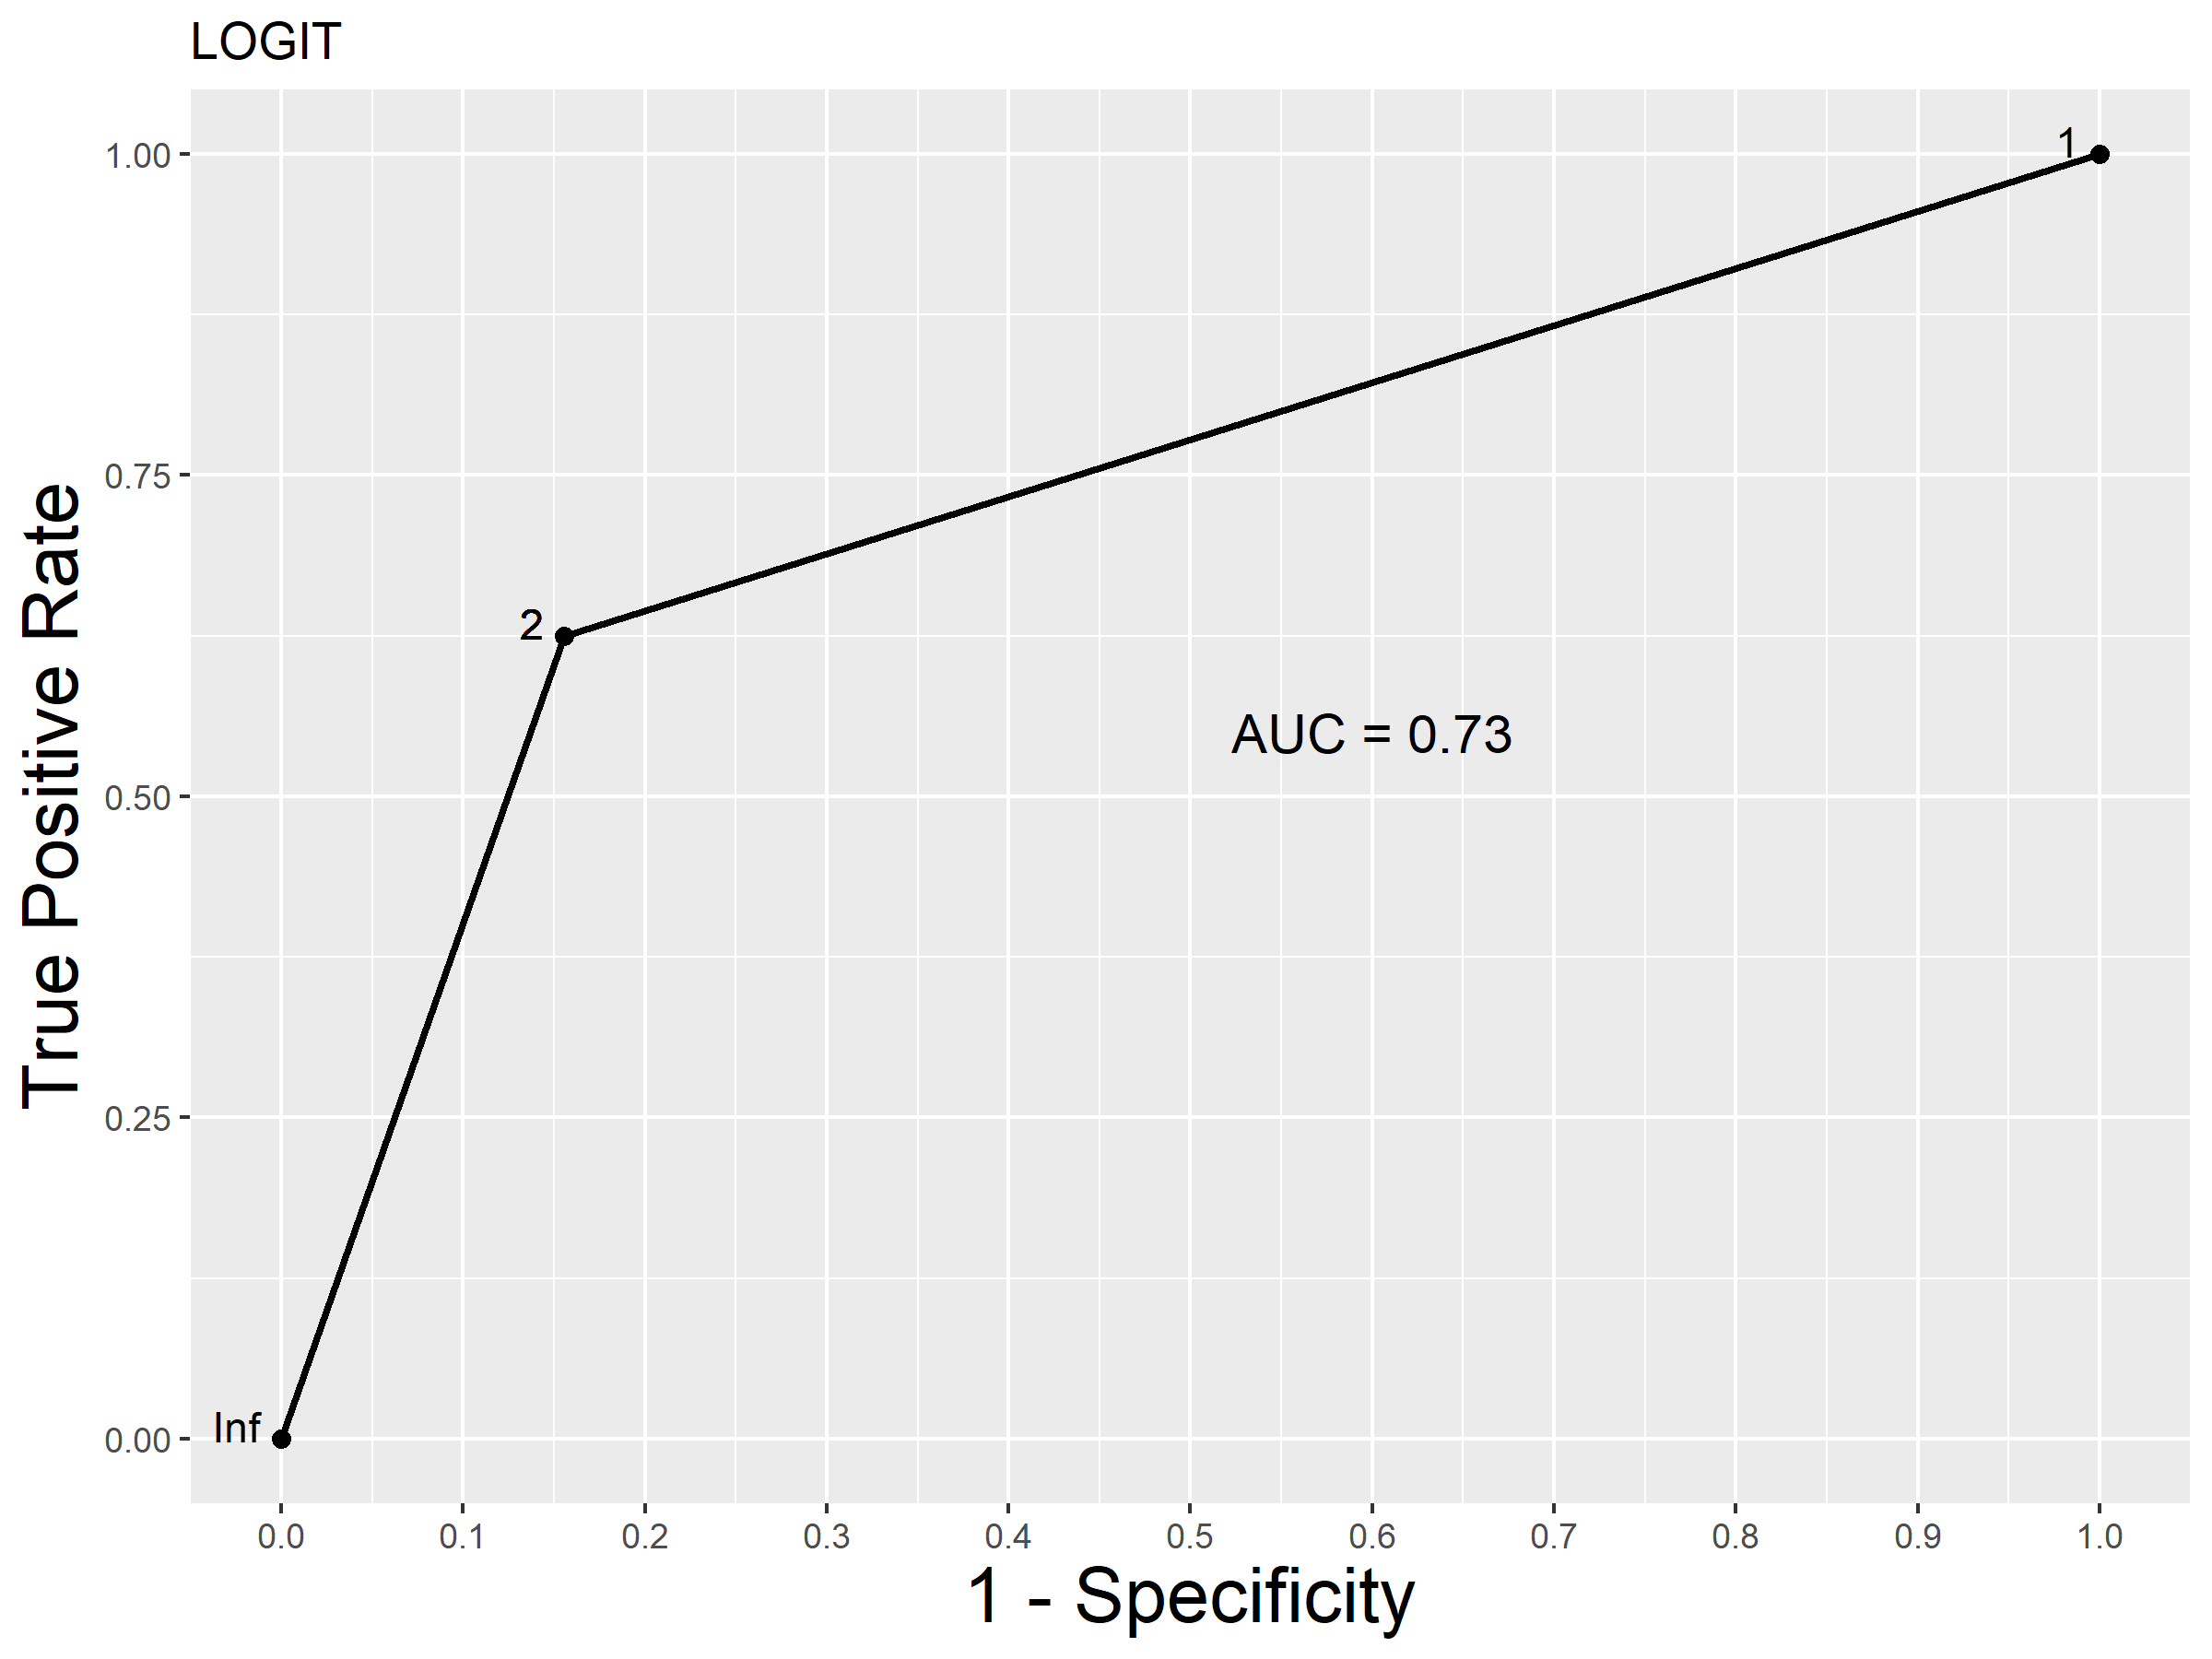
\includegraphics[width=0.45\linewidth]{logit}\quad
		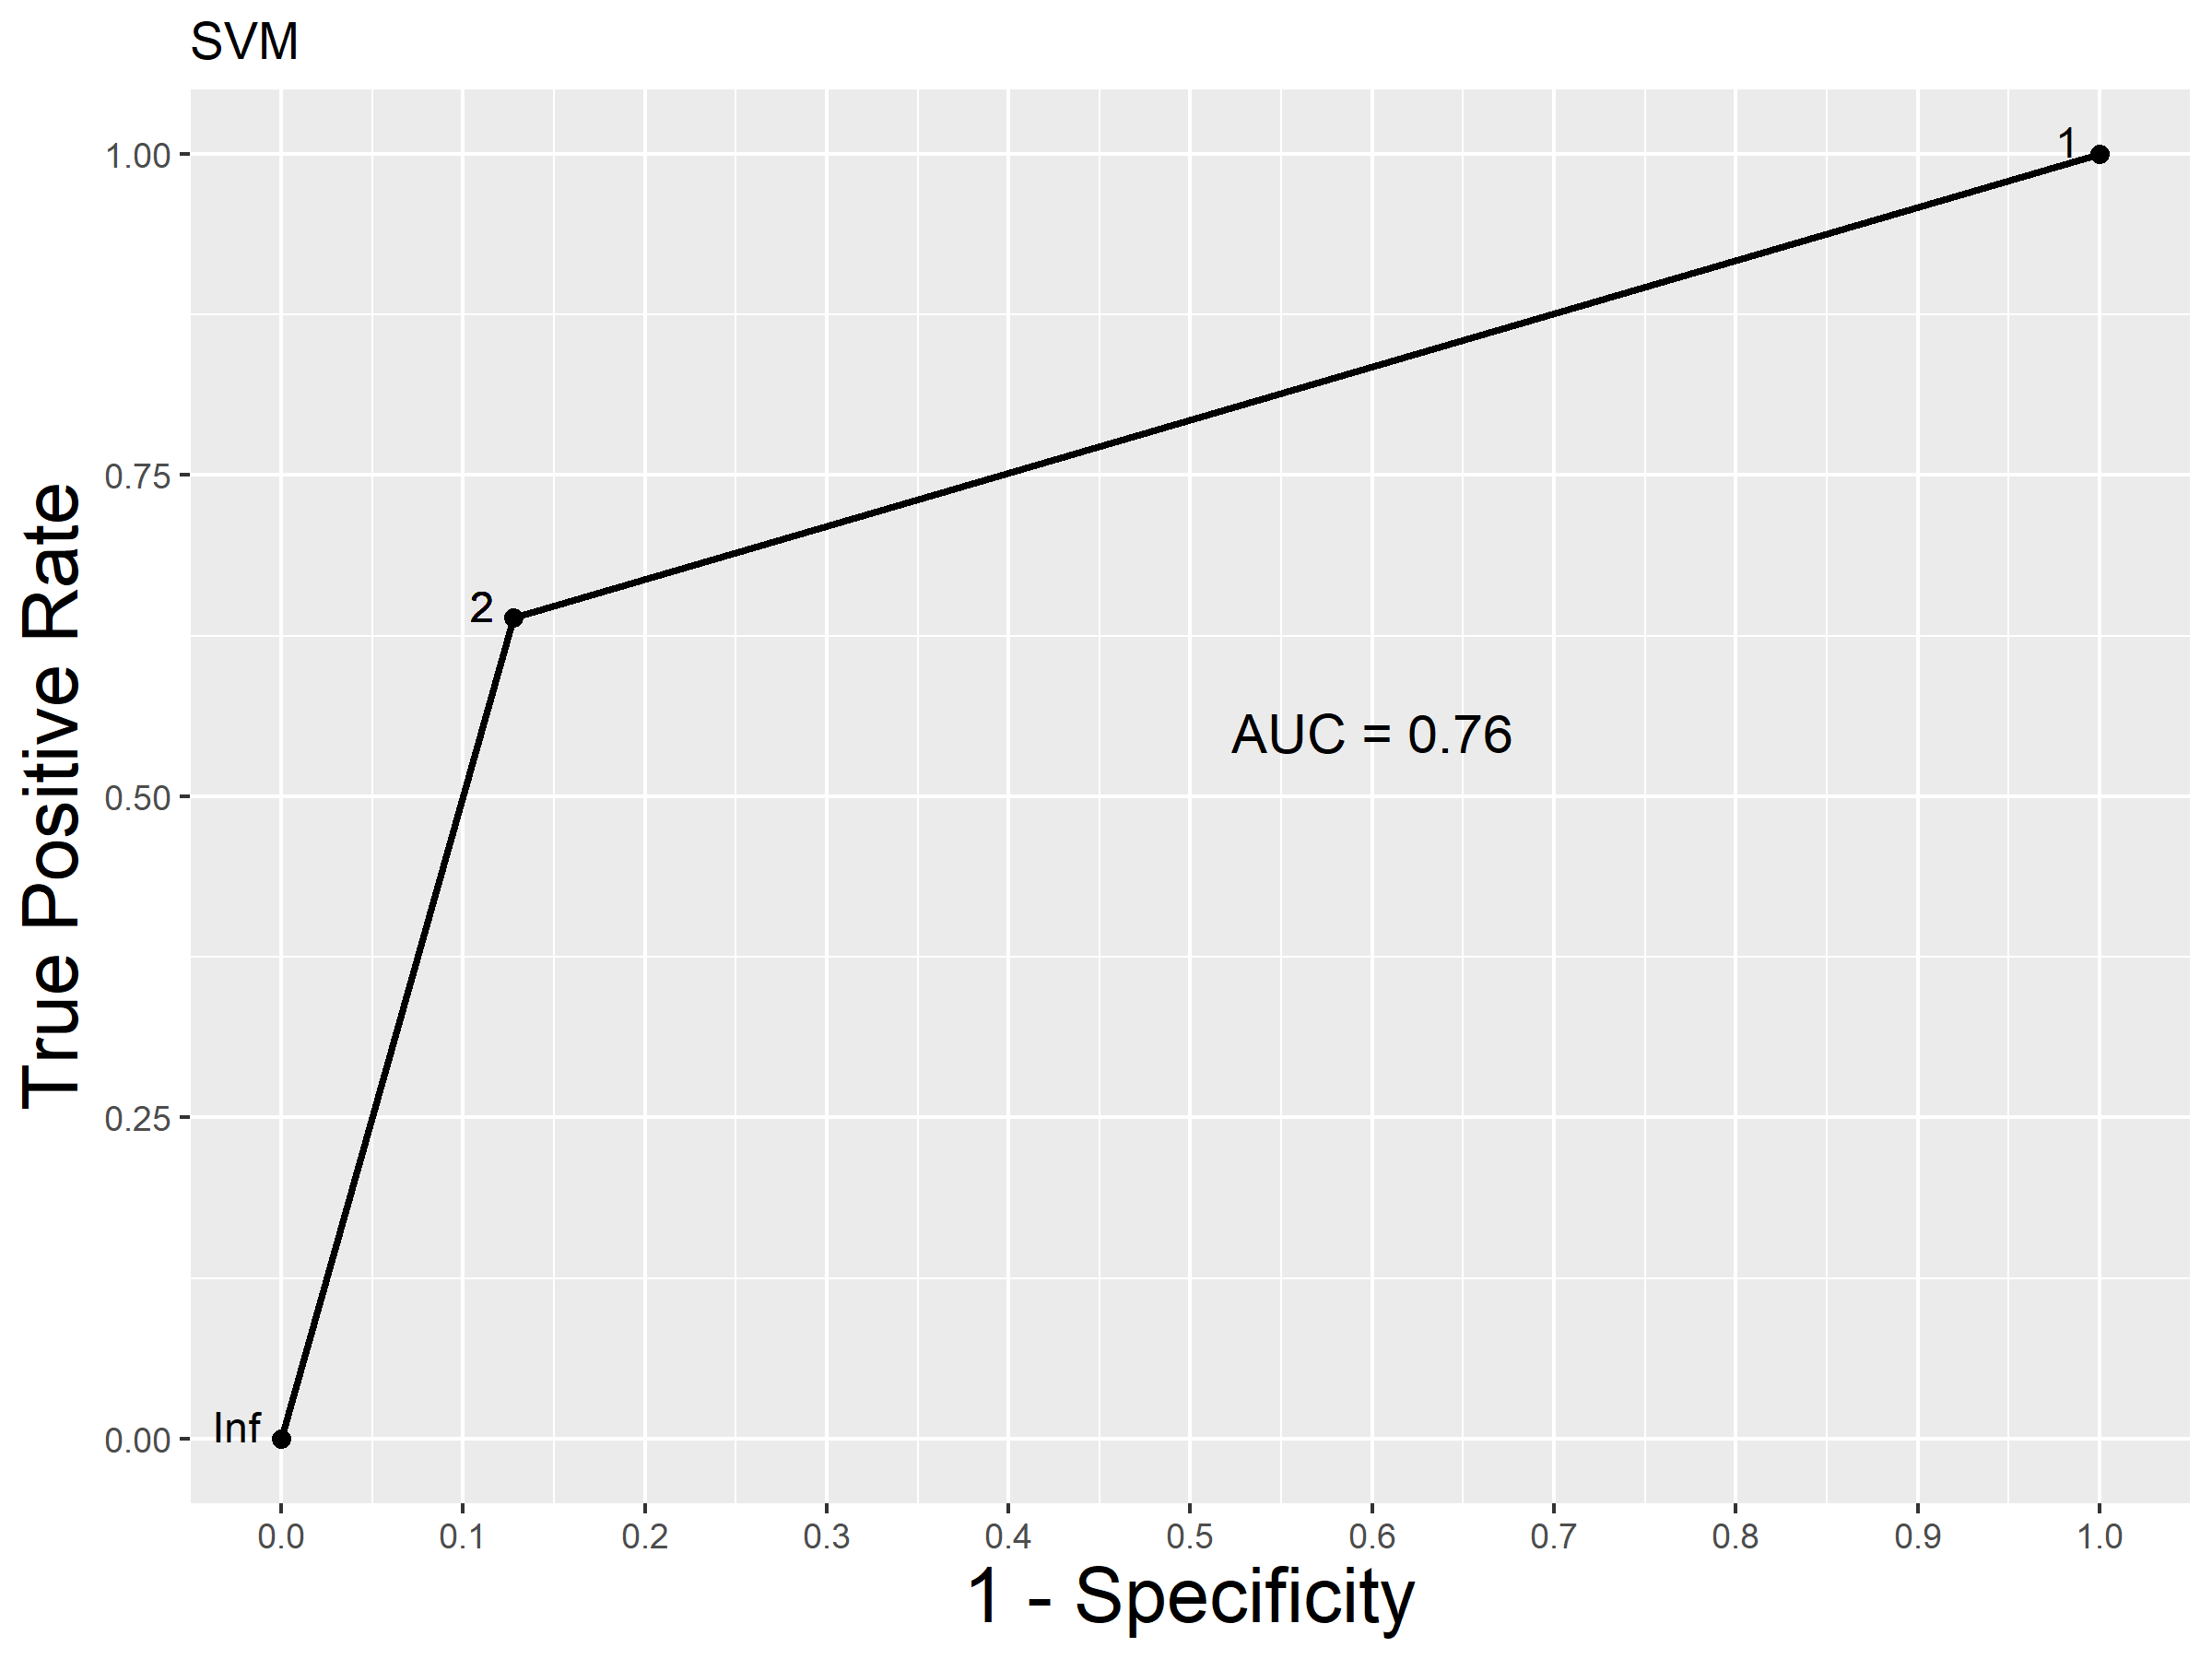
\includegraphics[width=0.45\linewidth]{svm}
		\caption{AUC: Logit and SVM}
		\label{fig:AUC1}
\end{figure}

\begin{figure}[H]
		\centering
		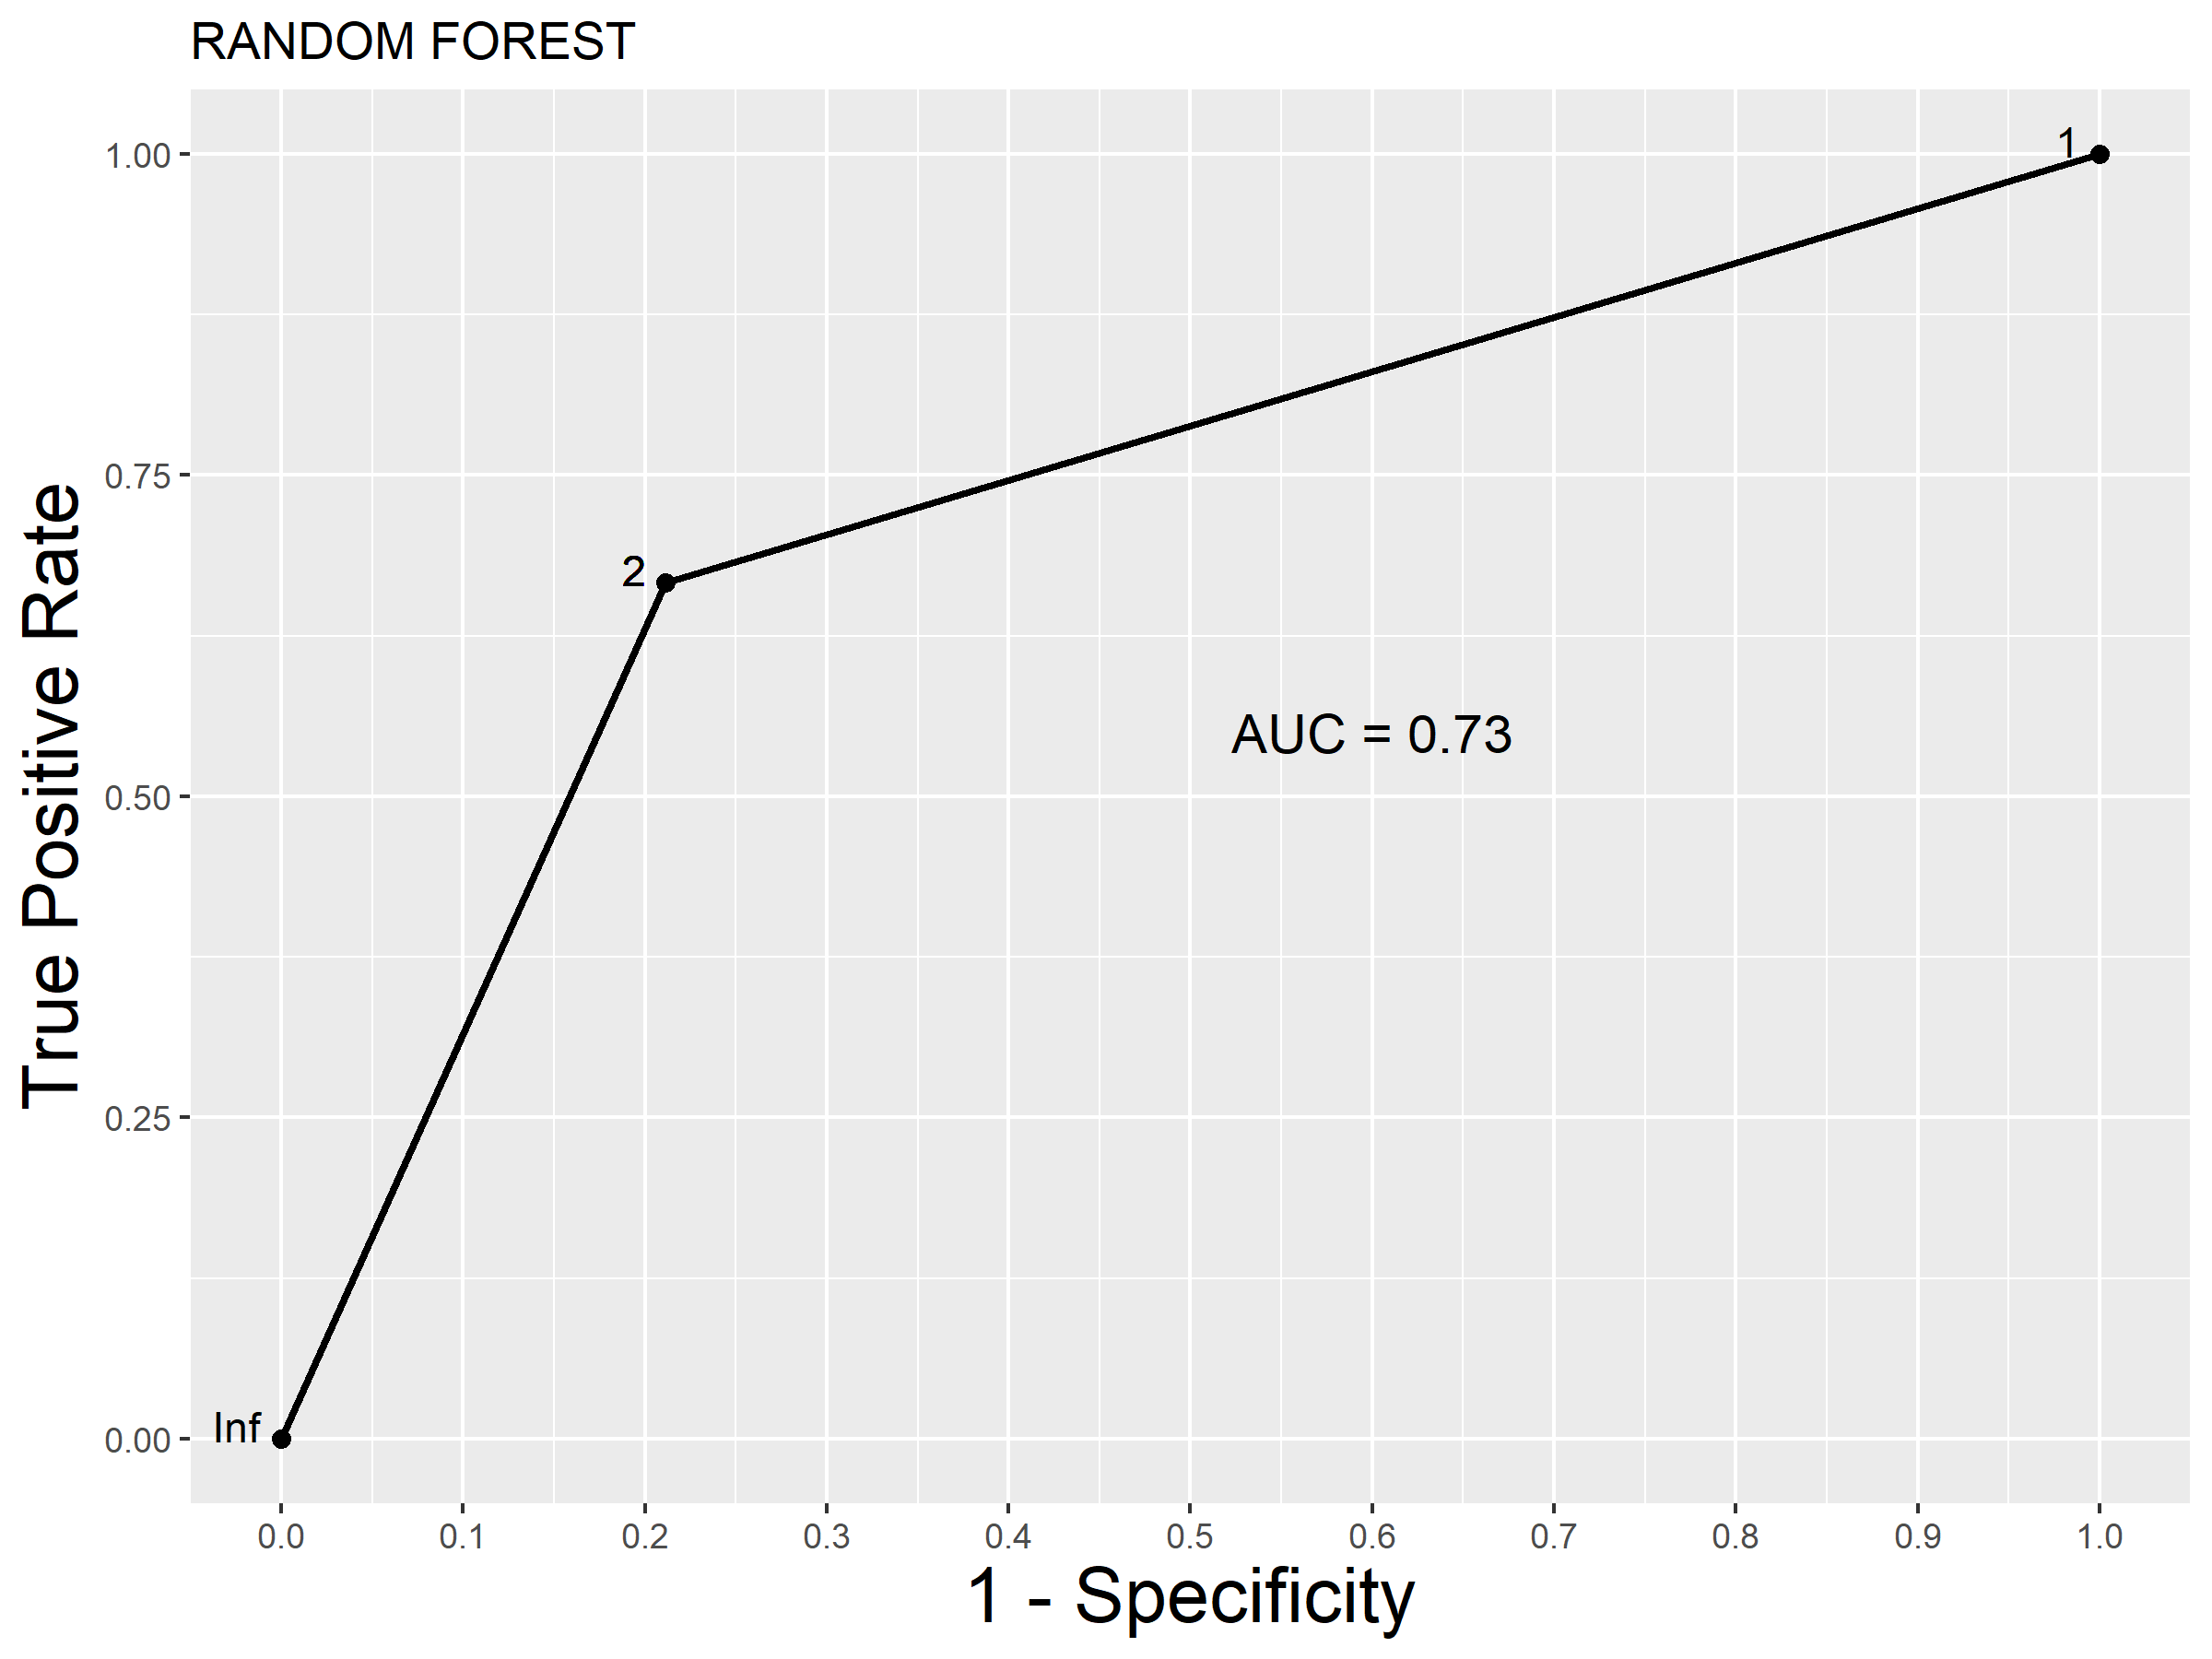
\includegraphics[width=0.45\linewidth]{RF}\quad
		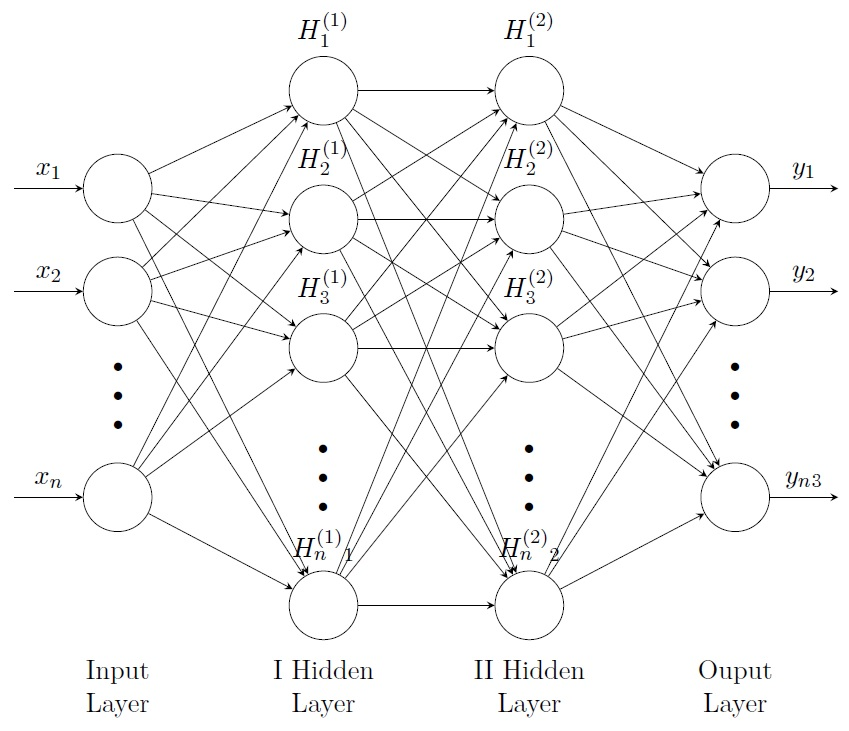
\includegraphics[width=0.45\linewidth]{nn}
\caption{AUC: Random Forest and Deep Neural Network}
		\label{fig:AUC2}
\end{figure}



\begin{table}[H]
\begin{center}

\begin{tabular}{c|c|c|c|c|c}
%\begin{tabular}{|c|c|c|c|c|}
\hline
\textbf{Model}          & \textbf{Accuracy}    &\textbf{AUC}  &  \begin{tabular}[c]{@{}c@{}}\textbf{McNemar's Test} \\ \textbf{P-Value}\end{tabular}  & \textbf{Sens.-Spec.}& \textbf{Kappa} \\ \hline
\multirow{ 2}{*}{\textbf{Logit}}         & 0.78        & 0.73 & 0.84452                & 0.864-0.588 & 0.460\\ 
               & (0.70-0.85) &      &                        &             \\ \hline
\multirow{ 2}{*}{\textbf{Random Forest}}      & 0.77        & 0.73 & 0.0045                 & 0.931-0.352 & 0.332 \\ 
               & (0.68-0.84) &      &                        &             \\ \hline
\multirow{ 2}{*}{\textbf{ SVM}}               & 0.80        & 0.76 & 0.83826                & 0.852-677 &  0.519  \\ 
               & (0.72-0.87) &      &                        &             \\ \hline
 \multirow{ 2}{*}{\textbf{Neural Network}}  & 0.73        & 0.67 & 0.98                   & 0.809-0.528 & 0.33 \\ 
               & (0.64-0.80) &      &                        &             \\ \hline
\end{tabular}
\end{center}
\caption{Model Performance: Random Forest and Deep Neural Network}
\label{Tab:2}
\end{table}

Table \ref{Tab:2} presents the statistics on the prediction performance in test data. Columns 2–6 show Accuracy, AUC, McNemar test, sensitivity-specificity, and Kappa estimators for each estimated model. 
We find that overall prediction accuracy ranges between 72\% and 80\% for our selected ML and Logit models, indicating the robustness of the sample. 
Furthermore, in each model true positive rates (sensitivity) exceed true negative rates (specificity), which means models perform better at detecting the target consumption behavior. We need to point out that Random Forest shows the McNemar test with a p-value <0.05, which means that the observed and predicted distribution differs from each other. This finds evidence also in a low Kappa and the highest sensitivity, expressed by Random Forest compared to other models, it seems specialized to detect positive examples.


%--------------------------------------------------------------------------------------------
\section{Discussion}
\label{sec:5}
%--------------------------------------------------------------------------------------------
\subsection{Consumer profiling}
\\
The consumer profile that emerges from our analysis is in line with the lifestyle patterns followed by urban young Chinese consumers. RTE salads' versatility contributes to maintaining a healthy lifestyle without giving up on taste and personalization.
Our results are consistent with studies conducted in other countries, but there are also significant differences regarding fresh-cut foods' consumption habits. 
Looking at the socio-demographic characteristics, similarly to our results, the literature on Western consumers found that the consumption is prevalent among females, middle-income earners, and individuals below forty years old (\cite{Massaglia19}; \cite{Sgroi18}; \cite{VanLoo10}). 
Our study also confirms the role of convenience as an essential purchasing factor (\cite{Stiletto20}; \cite{Vidal13}). The indicator "knowledge" was not significant in our model specification. Still, in its formulation, it aimed at capturing the role of objective information regarding RTE products, including food safety, quality, and freshness.
Regarding socio-demographic factors, our study is similar to the findings of a Korean study (\cite{Bae10}). Preferences for RTE products are significantly higher among young women who care about health. The similarities between the two realities might be associated with the so-called "Hallyu," the Korean wave, meaning South Korea's influence on other countries regarding lifestyles and consumer trends.
Another similarity is found with Indian consumers, who obtain information about RTE products through advertising (\cite{Hirekenchanagoudar08}). Another aspect worth mentioning is the role of subjective norms that is the degree of influence that other people exert on our choices. In our study, respondents giving importance to others' opinions are more likely to consume regularly RTE salads. This finding probably captures the awareness of how important it is to eat fresh vegetables to be healthy. In a collectivist society like China, following social rules is culturally vital for consensus and belonging. The importance of subjective norms in the Chinese context has been acknowledged in several behavioral studies. At the psychological level, it is, for example, adopted to reduce the perceived risk of adopting certain behaviors (\cite{Zhong21}), to increase self-preventive behaviors (\cite{Si21}), or to encourage sustainable choices, like waste recycling (\cite{Zhang15}).

As an additional contribution, this study provides new insights into the fresh-cut customers' behavior. Thereby using ML models, almost neglected in the analysis of consumer behavior, we offer a comprehensive perspective about predictive tasks, providing peculiar information for both policymakers and practitioners.
At first glance, it may seem surprising that our "non-ML" method would be comparable to our ML methods. 
The success of the logistic regression depends on how closely the conditional odds ratio can be approximated by a linear function. Indeed, our predictive investigation brings evidence that RF and DNN seem to not bring improvement to our predictions.  The latter seems to suffer from the lack of high data dimensionality, requiring more examples to achieve deep abstraction levels (see \cite{Lucun15}).
Our predictor sets have a relatively small number of covariates, and several of the predictors are binary, limiting the scope for model complexity and making it more likely that a simple linear model will yield an adequate approximation. With a larger pool of predictors, we might find that RF or DNN outperform our non-ML methods, which methods are likely to work best will depend on the pool of available predictor sets.
On the contrary, the marginal gain in prediction accuracy obtained when using the SVM is larger than other models, confirming the SVM ability as a powerful classifier.

Undoubtedly, the accuracy level would depend on the study context, to the best of our knowledge, literature does not provide a gold standard in predicting RTE  consumption behavior, even more in China market. Nevertheless, in the ML field, the 80\% of accuracy seems to be reasonable. We can therefore suggest that even in the field of consumer behavior a good combination of statistical modeling in lockstep with machine learning tools might be the best practice\footnote{Taking Kaggle competitions as a benchmark, a widespread platform among ML practitioners.} . In this way, it is possible to provide a reasonable solution to the trade-off between interpretability and better predictive performance.



\subsection{Conclusions}
This study's results are a preliminary contribution to an expanding food sector in China and have important policy implications. First, companies and institutions need to build communication campaigns to promote healthy eating habits among the population. Previous research in the literature showed how healthy marketing campaign towards RTE high-fiber cereals determined a significant growth in the purchasing level that lasted in the long term (\cite{Levy87}) Secondly, other reasons call for food regulator intervention within this market. A concern is, for example, the excessive use of plastic in the packaging (\cite{Tarancon21}). Consumers worldwide are becoming more sensitive to all the forms of pollution and prefer buying environmentally friendly products (\cite{Hartmann12}). Another criticism of fresh-cut fruits and vegetables is the high amount of waste food that, currently, the production process generates. However, there is evidence that the adoption of novel technologies can significantly reduce its amount (\cite{Plazzotta17}).  Finally, as mentioned above, RTE products are subject to contamination and spoilage if not properly handled (\cite{Evans16}). Therefore, recommending food safety practices for RTE products, such as refrigeration or eating instructions, is another important aspect that requires intervention from policymakers. 
It also highlighted the cold chain system, required in the transport of fresh cut products in a territory as large as that of China, which is certainly one of the factors that can facilitate the development of local companies. This can undoubtedly create additional entry barriers for international companies targeting to enter the promising Chinese fresh cut products market (\cite{ACE}).



\section{Appendix}

\subsection{Questions included in the analysis}
\label{App.Q}
\begin{enumerate} 
\item	Do you regularly consume (about 3 times per week) the RTE salads? 
\item	What is your gender?
\item	Please indicate your age range
\item	What is your highest level of completed education?
\item	What is your role within the company or organization you work for?
\item	How many people live in your household?
\item	How do you spend your free time? Fitness 
\item	Regarding RTE products, which statements do you think are true?
\item	RTE products must be washed before being consumed
Can be consumed directly
Are treated more than the fresh alternative
Are more healthy than the cool ones
Are industrial products very far from the quality of the fresh produce
Are more controlled and selected than the cool
\item	How did you learn about these products?
Advertising
Internet/social media/search engines
\item	Where do you usually buy RTE fresh-cut or packaged fruits and vegetables?
	Supermarket 
	Convenience Store
\item	When do you consume RTE products? (multiple options allowed)
Snacking 
Lunch 
\item	What is your family's opinion about cut and packaged products?
\item	What is your friends ' opinion about cut and packaged products?
\item	What is the opinion of your working/study colleagues on cut and packaged products?
\end{enumerate}


\subsection{Support Vector Machine}

Support Vector Machines originated as an altertinative to Neural Networks in the wide context of statistical learning, offering a solution to this trade-off by arbitrarily fixing model accuracy and minimising model complexity.\\ 
In a classification problem, this translates in an optimal solution identified by a linear hyperplane which correctly classifies observed data and lies as far as possible from them.\\

Consider the problem of binary classification or dichotomization. Considering the case of a two-dimensional input space, i.e., $\mathrm{x} \in \Re^{2} .$  Training data containing $l$ observation of two explanatory variable $X_1, X_2$ and the realisation of a target class $Y$,  are given as:
$$
\left(\mathrm{x}_{1}, y_{1}\right),\left(\mathrm{x}_{2}, y_{2}\right), \ldots,\left(\mathrm{x}_{l}, y_{l}\right), \mathrm{x} \in \Re^{n}, y \in\{+1,-1\}
$$

Data are linearly separable and we aim at find the optimal separating function (among many different hyperplanes) without knowing the underlying probability distribution $P(\mathrm{x}, y) .$

By using given training examples, during the learning stage, our machine finds parameters $\mathbf{w}=\left[w_{1} w_{2} \ldots w_{n}\right]^{T}$ and $b$ of (a discriminant) or decision function $d(\mathrm{x}, \mathrm{w}, b)$ given as
$$
d(\mathrm{x}, \mathrm{w}, b)=\mathrm{w}^{T} \mathrm{x}+b=\sum_{i=1}^{n} w_{i} x_{i}+b
$$
where $\mathbf{x}, \mathbf{w} \in \Re^{n}$, and the scalar $b$ is called $a$ bias. After the successful training stage, by using the weights obtained, the learning machine, given unseen pattern $\mathrm{x}_{p}$, produces output according to the following decision rule:

\begin{itemize}
\item if $d\left(\mathrm{x}_{p}, \mathrm{w}, b\right)>0,$ the pattern $\mathrm{x}_{p}$ belongs to $\{C_0\}\left(\right.$ i.e. $\left., o=y_{1}=+1\right)$  and
\item  if, $d\left(\mathrm{x}_{p}, \mathrm{w}, b\right)<0$ the pattern $\mathrm{x}_{p}$ belongs to $\{C_1\}\left(\right.$ i.e., $\left.o=y_{2}=-1\right)$.
\end{itemize}



Where $\{C_0, C_1\}$ are the two possible output classes and $b$ is a bias term.\\ Under these assumptions we define the setting outlined in Figure \ref{fig:marginsvm}, where the two dashed lines describe the so-called \textit{margin} to be maximised, which equals to
\begin{equation}\label{eq:margin}
    M = \min_{\textbf{x}:y=1}\frac{\textbf{wx}}{||\textbf{w}||} - \max_{\textbf{x}:y=-1}\frac{\textbf{wx}}{||\textbf{w}||},
\end{equation}

\begin{figure}[h]
    \centering
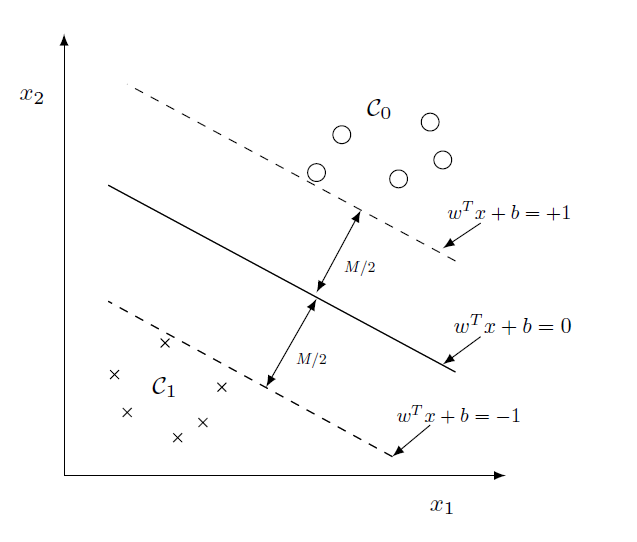
\includegraphics[width=0.5\linewidth]{svm_model}
\caption{\label{fig:marginsvm} SVM decision boundary and margin.}
\end{figure}


Since from the decision rule and (\ref{eq:margin}) follows that
\begin{equation}
    M = 2\frac{|\textbf{wx}|}{||\textbf{w}||} = \frac{2}{||\textbf{w}||}
\end{equation}
that is a geometrical translation of margins.
Therefore we can write the SVM optimisation problem as
\begin{equation}\begin{split}\label{eq:softmarginsvm}
&\min \quad \frac{1}{2}\textbf w^T\textbf w\\
&sub \quad  y_n[\textbf w^T\textbf x_n + b]\ge 1\quad \forall n=1, \dots, N
\end{split}\end{equation}

This is a classic quadratic optimization problem with inequality constraints. Such an optimization problem is solved by the saddle point of the
Lagrange functional (Lagrangian):

$$
L(\mathbf{w}, b, \alpha)=\frac{1}{2} \mathbf{w}^{T} \mathbf{w}-\sum_{n=1}^{N} \alpha_{i}\left\{y_{n}\left[\mathbf{w}^{T} \mathbf{x}_{i}+b\right]-1\right\}
$$
where the $\alpha_{i}$ are Lagrange multipliers. The search for an optimal saddle point $\left(\mathrm{w}_{0}, b_{0}, \alpha_{0}\right)$ is necessary because Lagrangian $L$ must be minimized with respect to $\mathrm{w}$ and $b$, and has to be maximized with respect to nonnegative $\alpha_{i}$ (i.e., $\alpha_{i} \geq 0$ should be found). %This problem can be solved either in a primal space (which is the space of parameters $\mathbf{w}$ and $b$ ) or in a dual space (which s the space of Lagrange multipliers $\alpha_{i}$ ). The second approach gives insighttul results and we will consider the solution in a dual space below. In order o do that, we use Karush-Kuhn-Tucker (KKT) conditions for the optimum of a constrained function. 
%
\subsection{Deep Neural Network}

%The term NN refers to a mathematical model inspired by the human brain. It allows computational models composed of multiple processing layers to learn representations of data characterized by multiple levels of abstraction, solving even the most complex problems. Its architecture includes neurons, synaptic connections that link the neurons, and learning algorithms (backpropagation). NN works as a weighted regression in which each unit gets “weighted” information through synaptic links from the other connected ones, returning an output by using an activation function that transforms the weighted sum of input signals. Albeit DL embodies a broad variety of networks differing from each other by the architectural structure, in this section the basic scheme of NN has been presented, the so-called feedforward structure.

%In the feedforward framework, the information moves from the input to the output layer in only one direction. At the same time, Recurrent Neural Networks (RNNs), used in chapter 5, leverage on recurrent structure processing information cyclically. They are characterized by self-connected units or connected to units of the previous layers (in addition to the feedforward connections).
%Fig.\ref{schemaNN} shows the schematical view of feedforward NN. The circles represent neurons and lines represent synapses.
%Synapses take the input and multiply it by a “weight” (the “strength” of the input in determining the output).
%Neurons add the outputs from all synapses and apply an activation function.

%\begin{figure}[htbp]
%\begin{center}
%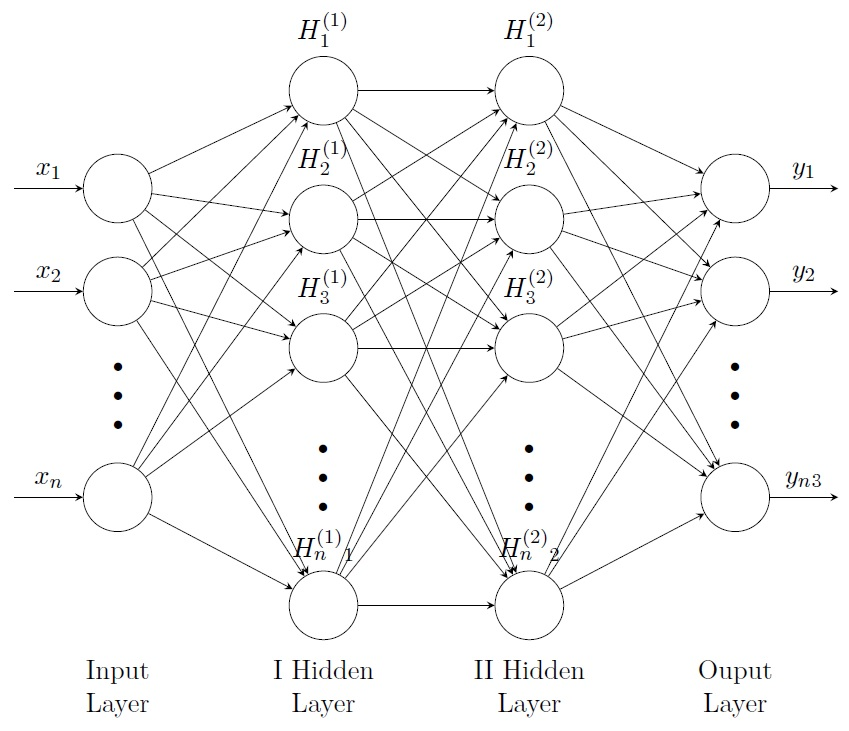
\includegraphics[width=\textwidth]{nn}
%\caption{Schematic view of feedforward NN}
%\label{schemaNN}
%\end{center}
%\end{figure}

NN training involves an unconstrained optimization problem where the aim is to minimize a
function in high dimensional space the so-called loss function, that measures the difference between the predicted values and observed ones.
The back-propagation is the most used algorithm for the training of NNs. The algorithm compares the predicted values against the desired ones (objective)
and modifies the synaptic weights by back-propagating the gradient of the loss function. Schematically,
the procedure alternates forward and backward propagation steps:
\begin{itemize}
\item in the forward step, the prediction is computed fixing the synaptic weights,
\item in the backward step, the weights are adjusted in order to reduce the error of the network.
\end{itemize}
The NN iteratively performs forward and backward propagation and modifies the weights to
find the combination that minimizes the loss function $\mathcal{L}$.

It is possible to formally describe the forward pass, to aim at obtaining the target output. Specifically, we have the activation function $f^k$, weights matrix $W^{(k)}$, hidden layers $H^{(k)}$
%The following equations detailed describes NN structure and forward pass for the first hidden layer.
%\begin{equation}
%\begin{cases}
%H_1^{(1)}=f^1 \Big( x_1\,\omega^{(1)}_{1,1}+x_2\,\omega^{(1)}_{1,2}+x_3\,\omega^{(1)}_{1,3}+ \dots+x_n\,\omega^{(1)}_{1,n}+b_{1,1}\Big)\\
%H_2^{(1)}=f^2\Big(x_1\,\omega^{(1)}_{2,1}+x_2\,\omega^{(1)}_{2,2}+x_3\,\omega^{(1)}_{2,3}  +\dots+x_n\,\omega^{(1)}_{2,n}+b_{1,2}\Big)\\
%H_3^{(1)}=f^3\Big(x_1\,\omega^{(1)}_{3,1}+x_2\,\omega^{(1)}_{3,2}+x_3\,\omega^{(1)}_{3,3}  +\dots+x_n\,\omega^{(1)}_{3,n}+b_{1,3}\Big)\\
%\dots\\

%H_{n1}^{(1)}=f^{n-1}\Big(x_1\,\omega^{(1)}_{n_1,1}+x_2\,\omega^{(1)}_{n_1,2}+x_3\,\omega^{(1)}_{n_1,3}+\dots+x_n\,\omega^{(1)}_{n_1,n}+b_{1,n}\Big)\\
%\end{cases}
%\end{equation}
%\\
%For the second hidden layer
%\begin{equation}
%\begin{cases}
%H_1^{(2)}=f^1\Big(H_1^{(1)}\omega^{(2)}_{1,1}+H_2^{(1)}\omega^{(2)}_{1,2}+H_3^{(1)}\omega^{(2)}_{1,3} +\dots+H_{n1}^{(1)}\omega^{(2)}_{1,n1}+b_{2,1}\Big)\\
%H_2^{(2)}=f^2\Big(H_1^{(1)}\omega^{(2)}_{2,1}+H_2^{(1)}\omega^{(2)}_{2,2}+H_3^{(1)}\omega^{(2)}_{2,3}+\dots+H_{n1}^{(1)}\omega^{(2)}_{2,n1}+b_{2,2}\Big)\\
%H_3^{(2)}=f^3\Big(H_1^{(1)}\omega^{(2)}_{3,1}+H_2^{(1)}\omega^{(2)}_{3,2}+H_3^{(1)}\omega^{(2)}_{3,3}+\dots+H_{n1}^{(1)}\omega^{(2)}_{3,n1}+b_{2,3}\Big)\\
%\dots\\
%H_{n_2}^{(2)}=f^{n2}\Big(H_1^{(1)}\omega^{(2)}_{n2,1}+H_2^{(1)}\omega^{(2)}_{n2,2}+H_3^{(1)}\omega^{(2)}_{n2,3}+\dots+H_{n1}^{(1)}\omega^{(2)}_{n2,n1}\!+b_{2,n1}\Big)\\
%\end{cases}
%\end{equation}
 
where $\mathbf{X}$ e $\mathbf{W^{(k)}}$ are respectively, input and weights vectors and $\mathbf{b}$ the bias column. Thus for the $k$-th hidden layer $\mathbf{H^{(k)}}$ :
\begin{equation}
\mathbf{H^{(k)}}=f^k\big(\mathbf{W^{k}\,H^{(k-1)}}+\mathbf{b^{(k)}}\big)
\end{equation}

and thus, we can rewrite as function of the input $\mathbf{X}$:

\begin{equation}
\mathbf{H^{(k)}}=f^{(k)}\big(\mathbf{W^{(k)}}\,    \underbrace{f^{(k-1)} \big(	\dots f^{(1)}\big(\mathbf{W^{1}\,\mathbf{X}}+\mathbf{b^{(1)}}\big)\dots\big)}_%
{=\mathbf{H^{(k-1)}}}		 +\mathbf{b^{(k)}}\big)
\end {equation}
 
After the estimation procedure, which implies to estimate the weights, we obtain the final output, $\hat{y}$, resulting from the application of the DNN parameters (weights matrix $\mathbf{\hat{W}}$ and bias $\mathbf{\hat{b}}$) obtained by the optimization procedure described in the following.\\
NN, like other machine learning techniques, requires the splitting of the dataset into a training and a testing set. The training set stands for supervised learning, while the testing set is used to
validate the model. After the training phase, the network has learned the input–output functional relationship and it should be able to predict future values using only the input.
Practically, NN parameters are obtained by the minimization of the overall loss function $\mathcal{L}$. In the classification problem the most widely used loss function is the binary cross-entropy:
%$$\mathcal{L}(log[\mathbf{M_{(a,t)}}],log[\mathbf{\hat{M}_{(a,t)}}]) = \frac{1}{a \cdot t}\sum_{a,t}\left(log[\mathbf{M_{(a,t)}}]-log[\mathbf{\hat{M}_{(a,t)}}]\right)^2$$
$$\mathcal{L}(y,\hat{y})=-\sum_{i=1}^{n} y_{i} \log \hat{y}_{i}+\left(1-y_{i}\right) \log \left(1-\hat{y}_{i}\right)$$

%$$\mathcal{L}(y,\hat{y}) = \frac{1}{n}\sum_{i=1}^{n}\left(y_i-\hat{y}_i\right)^2$$
To minimize the loss function, we use the Gradient Descent optimization algorithm, which iteratively moves in the direction of steepest descent as defined by the negative of the gradient.

This algorithm proceeds by minimizing $\mathcal{L}$ at each step $t$,  therefore differentiating the loss function with respect to the weights  ($\mathbf{{W}}$).
%\begin{equation}
%\nabla  \mathcal{L}(y,\hat{y})=
%\begin{bmatrix}
%\frac{\partial \mathcal{L}(y,\hat{y})}{\partial w_{1,1}^{(1)}}\\
%\frac{\partial \mathcal{L}(y,\hat{y})}{\partial w_{1,2}^{(1)}}\\
%\frac{\partial \mathcal{L}(y,\hat{y})}{\partial w_{1,3}^{(1)}}\\
%\vdots \\
%\frac{\partial \mathcal{L}(y,\hat{y})}{\partial w_{n,n}^{(k)}}\\
%\end{bmatrix}
%\end{equation}
For the generic weights $w_{n,n}^{(k)}$ and the $k$-th layer, the algorithm proceeds using the chain derivation rule described in the following equation:
\begin{equation}
\frac{\partial \mathcal{L}(y,\hat{y})}{\partial w_{n,n}^{(k)}} =\frac{\partial \mathcal{L}(y,\hat{y})}{\partial H_n^{(k)}}\,\frac{{\partial H_n^{(k)}}}{\partial z_n^{(k)}} \, \frac{\partial z_n^{(k)}}{\partial w_{n,n}^{(k)}}
 \end{equation}
where $ z_n^{(k)}=w_{n}^{(k)}\,H_{n}^{(k-1)}+b_n^{(k)}$. 
To update the weights ($\mathbf{\tilde{W}}$), the gradient of the loss function, $\nabla \mathcal{L}_t(y,\hat{y})$, is multiplied by a scalar, $\eta$, often called learning rate, according to the following scheme:

\begin{equation}
\mathbf{\tilde{W}}=\mathbf{W}-\eta \nabla \mathcal{L}_t(y,\hat{y})
\end{equation}
In a figurative way, the idea behind the gradient descent is similar to “climbing down a hill” until a global or local minimum is reached. At each update, the search moves in the opposite direction of the gradient and the learning rate $\eta$ determines the amplitude of this movement, controlling the adjustment in the weights, thus determining how fast or slow we will move towards the optimal weights.
A very large learning rate leads to a sub-optimal solution. A very small learning rate involves too many iterations to find the optimal solution. 
Then, the learning rate can be considered the most important hyper-parameter for tuning NN.

The search for the optimal parameters is then carried out through an optimization process where the NN initial weights are selected in an arbitrary (random) way so they are not optimal parameters. The iterations of the algorithm lead to the optimization of the weights and minimization of the error. 
The choices concerning the type of architecture (e.g., the number of hidden layers, units for each layer) and the hyperparameter (e.g., learning rate, activation functions, and loss function), remains a heuristic problem for NN users: the choice often depends on the type of data and it is not an easy step. 



\subsection{Random Forest}

%The RF algorithm constructs a multitude of decision trees at training time with bootstrapping and randomly chosen predictors, and then aggregates them for final prediction. Tree models without randomization may produce weak predictions if the trees are correlated (Hastie et al., 2009, p.587). RF grows each tree to a resampled part of the data, which makes the trees different and de-correlates them. RF offers better comprehension than neural-network-type algorithms for its tree-like structure, hence it is gaining use in the social sciences (e.g. Davis and Heller, 2017 ).




%\pragraph{Regression Tree Architecture}
%The random forest algorithm is founded on the regression tree architecture. The regression trees enable attaining the best function approximation $\hat{f}\left(X_{1}, X_{2}, \ldots, X_{p}\right)$ through a procedure consisting in the following steps Loh (2011):

%The predictor space (i.e., the set of possible values for $\left.X_{1}, X_{2}, \ldots, X_{p}\right)$ is divided into $J$ distinct and non-overlapping regions, $R_{1}, R_{2}, \ldots, R_{J}$ For each observation that falls into the region $R_{j}$, the algorithm provides the same prediction, which is the mean of the response values for the training observations in $R_{j}$.

%As described in James et al. (2017), the fundamental concept is to split the predictors' space into rectangles, identifying the regions $R_{1}, \ldots, R_{J}$ that minimize the Residual Sum of Squares (RSS):
%$$
%\sum_{j=1}^{J} \sum_{i \in R_{j}}\left(y_{i}-\hat{y}_{R_{j}}\right)^{2}
%$$
%Once building the regions $R_{1}, \ldots, R_{J}$, the response is predicted for a given test observation using the mean of the training observations in the region to which that test observation appertain.

%The consideration of all the possible partitions of the feature is computationally infeasible, thus we use a top-down approach through a recursive binary partition Quinlan (1986): the algorithm starts at the top of the tree, where all values of the target variable stand in a single region, and then successively partitions the predictors' space. The best split is identified according to the entropy or the index of Gini that is a homogeneity measure for every node. The highest homogeneity (or purity) is achieved when only one class of the target variable is attending the node.

%Breiman (2001) has listed the most interesting properties of regression tree-based methods. They belong to non-parametric methods able to catch tricky relations between inputs and outputs, without involving any a-priori assumption. They manage miscellaneous data by applying features selection so as to be robust to not significant or noisy variables. They are also robust to outliers or missing values and easy to be unfolded.


The random forest (RF) algorithm creates a collection of decision trees from a casually variant of the tree. Once one specific learning set is defined, the RF presents a random perturbation to the learning procedure and in this way a differentiation among the trees is produced. Successively the predictions of all these trees is derived through the impelementation of aggregation techniques. The first aggregation procedure was described by \cite{Breiman96}; the authors proposed the well know bagging based on random bootstrap copies of the original data to assemble different trees. Later in 2001 the same authors \cite{Breiman01}r proposed the random forest as an extention of the procedure of the bagging such that it combines the bootstrap with randomization of the input variables to separate internal nodes $t$. This means that the algorithm does not identify the best split $s_{t}=s^{*}$ among all variables, but firstly creates a random subset of $K$ variables for each node and among them determines the best split.

The RF estimator, for both regression and classification problem, of the target variable $\hat{y}_{R_{j}}$ is a function of the regression or classification tree estimator, $f^{\text {tree }}(\mathbf{X})=$ $\sum_{j \in J} \hat{y}_{R_{j}} \mathbf{1}_{\left\{\mathbf{X} \in R_{j}\right\}}$, where $\mathbf{X}=\left(X_{1}, X_{2}, \ldots, X_{p}\right)$ is the vector of the predictors, $\mathbf{1}_{\{-\}}$ represents the indicator
function and $\left(R_{j}\right)_{j \in J}$ are the regions of the predictors space obtained by minimizing the binary cross entropy Loss Function %\footnote{the $\mathrm{RSS}=\sum_{}^{}\left(Y_{}-f\left(X_{}\right)\right)^{2}$ for regression problem, and $L(Y, f(X))=I(Y \neq f(X))=$\left\{\begin{array}{c}
%0 \text { if } Y=f(X) \\
%1 \text { otherwise }
%\end{array}\right.}\\ for a binary target variable.}
%It is identified by the average values of the variable belonging to the same region $R_{j}$.
Therefore, denoting the number of bootstrap samples by $B$ and the decision tree estimator developed on the sample $b \in B$ by $\hat{f}^{\text {tree }}(\mathbf{X} \mid b)$, the RF estimator is defined as follows:
$$
f^{R F}(\mathbf{x})=\frac{1}{B} \sum_{b=1}^{B} f^{\operatorname{tree}}(\mathbf{X} \mid b)
$$




%--------------------------------------------------------------------------------------------
% 
%--------------------------------------------------------------------------------------------
\begin{thebibliography}{999}

\bibitem[Acock (2008)]{Acock08}
Acock, A. C. (2008). A gentle introduction to Stata. Stata press.

\bibitem[Artes et al. (2019)]{Artes}	
Artés, F., Gómez, P., Aguayo, E., Escalona, V., & Artés-Hernández, F. (2009). Sustainable sanitation techniques for keeping quality and safety of fresh-cut
plant commodities. Postharvest Biology and Technology, 51(3), 287–296.


\bibitem[Bae et al. (2010)]{Bae10}
Bae, H.-J., Chae, M.-J., & Ryu, K. (2010). Consumer behaviors towards ready-to-eat foods based on food-related lifestyles in Korea. Nutrition Research and Practice, 4(4), 332.

\bibitem[Baselice et al. (2017)]{Baselice17}
Baselice, A., Colantuoni, F., Lass, D. A., Nardone, G., & Stasi, A. (2017). Trends in EU consumers’ attitude towards fresh-cut fruit and vegetables. Food Quality and Preference, 59, 87-96.

\bibitem[Bischl et al. (2012)]{Bischl12}
Bischl, B., Mersmann, O., Trautmann, H., & Weihs, C. (2012). Resampling methods for meta-model validation with recommendations for evolutionary computation. Evolutionary computation, 20(2), 249-275.

\bibitem[Brennan et al. (2013)]{Brennan13}
Brennan, M. A., Derbyshire, E., Tiwari, B. K., & Brennan, C. S. (2013). Ready to eat snack products: The role of extrusion technology in developing consumer acceptable and nutritious snacks. International Journal of Food Science \& Technology, 48(5), 893–902.

\bibitem[Breiman (1996)]{Breiman96}
Breiman, L. (1996). Bagging predictors. Machine learning 24 (2), 123-140

\bibitem[Breiman (2001)]{Breiman01}
Breiman, L. (2001). Random forests. Machine learning 45 (1), 5-32

\bibitem[Buckley et al. (2007)]{Buckley07}
Buckley, M., Cowan, C., & McCarthy, M. (2007). The convenience food market in Great Britain: Convenience food lifestyle (CFL) segments. Appetite, 49(3), 600-617.

\bibitem[Cassady et al. (2007)]{Cassady07}
Cassady, D., Jetter, K. M., & Culp, J. (2007). Is price a barrier to eating more fruits and vegetables for low-income families?. Journal of the American Dietetic Association, 107(11), 1909-1915.

\bibitem[Cohen (1960)]{Cohen60}
Cohen J. (1960). A Coefficient of Agreement for Nominal Scales. Educational and Psychological Measurement. 20(1):37-46. 

%\bibitem[Commission Regulation]{CommReg}
%Regulation 2073/2005/EC. (n.d.). Commission Regulation EC No 2073/2005. Microbiological criteria for foodstuffs. OJ.J. \url{http://data.europa.eu/eli/reg/2005/2073/oj}

\bibitem[China Nutrition Improvement Action Plan (1996-2000)]{ActionPlan}
The State Council of China. China Nutrition Improvement ActionPlan (1996-2000). The State Council of China, Beijing; 1997.

\bibitem[Chonpracha et al. (2020)]{Chonpracha20}
Chonpracha, P., Ardoin, R., Gao, Y., Waimaleongora-Ek, P., Tuuri, G., & Prinyawiwatkul, W. (2020). Effects of intrinsic and extrinsic visual cues on consumer emotion and purchase intent: A case of ready-to-eat salad. Foods, 9(4), 396.

\bibitem[Daxue Consulting (2021)]{DaxueConsulting21}
Daxue Consulting. (2021). Survey on Health Perceptions in China. \url{https://daxueconsulting.com/health-perceptions-in-china/}

\bibitem[Dinnella et al. (2014)]{Dinnella14}
Dinnella, C., Torri, L., Caporale, G., & Monteleone, E. (2014). An exploratory study of sensory attributes and consumer traits underlying liking for and perceptions of freshness for ready to eat mixed salad leaves in Italy. Food Research International, 59, 108–116.

\bibitem[ Evans\& Redmond (2016)]{Evans16}
Evans, E. W., & Redmond, E. C. (2016). Older adult consumer knowledge, attitudes, and self-reported storage practices of ready-to-eat food products and risks associated with listeriosis. Journal of Food Protection, 79(2), 263–272.

\bibitem[F. A. O. (2017)]{FAO17}
Faostat, F. A. O. (2017). Available online: \url{http://www.fao.org/faostat/en/#data}. QC (accessed on January 2020).

\bibitem[Frewer et al. (2013)]{Frewer13}
Frewer, L. J., Risvik, E., & Schifferstein, H. (Eds.). (2013). Food, people and society: a European perspective of consumers' food choices. Springer Science & Business Media.

\bibitem[Gibson\&Partridge (2019)]{Gibson19}
Gibson, A. A., & Partridge, S. R. (2019). Nutritional qualities of commercial meal kit subscription services in Australia. Nutrients, 11(11), 2679.

\bibitem[Gibson et al. (2012)]{Gibson12}
Gibson, A., Edgar, J. D., Neville, C. E., Gilchrist, S. E., McKinley, M. C., Patterson, C. C., Young, I. S., & Woodside, J. V. (2012). Effect of fruit and vegetable consumption on immune function in older people: A randomized controlled trial. The American Journal of Clinical Nutrition, 96(6), 1429–1436.

\bibitem[Gordon et al. (2006)]{Gordon06}
Gordon, R., McDermott, L., Stead, M., & Angus, K. (2006). The effectiveness of social marketing interventions for health improvement: what's the evidence?. Public health, 120(12), 1133-1139.

\bibitem[Glorot and Bengio (2011)]{Glorot}
Glorot, X. and Bengio, A. B. . Y. (2011). Deep sparse rectifier neural networks. In Gordon, G.,Dunson, D., and Dudík, M., editors, Proceedings of the Fourteenth International Conference on Artificial Intelligence and Statistics, volume 15 of Proceedings of Machine Learning Research, pages 315–323, Fort Lauderdale, FL, USA. JMLR Workshop and Conference Proceedings

\bibitem[Gu et al. (2021)]{Gu21}
Gu, Y., He, Y., Ali, S. H., Harper, K., Dong, H., & Gittelsohn, J. (2021). Fruit and Vegetable Intake and All-Cause Mortality in a Chinese Population: The China Health and Nutrition Survey. International Journal of Environmental Research and Public Health, 18(1), 342.

\bibitem[Hansstein et al. (2017)]{Hansstein17}
Hansstein, F., Keqiang, W., & Hongmei, L. (2017). Perceptions of food quality: Evidence from a survey in Shanghai. International Journal of Consumer Studies, 41(6), 754–760.

\bibitem[Hartmann \& Apaolaza-Ibáñez (2012)]{Hartmann12}
Hartmann, P., & Apaolaza-Ibáñez, V. (2012). Consumer attitude and purchase intention toward green energy brands: The roles of psychological benefits and environmental concern. Journal of Business Research, 65(9), 1254–1263.

\bibitem[Hastie, T., Tibshirani, R. and Friedman, J. (2009)]{Hastie16}
Hastie, T., Tibshirani, R.  and Friedman, J.The Elements of Statistical Learning. Springer Series in Statistics Springer New York Inc., New York, NY, USA, (2009)

\bibitem[Healthy China Action Plan (2019–2030)]{HCAP}
The State Council of China. Healthy China Action Plan (2019–2030). The State Council of China, Beijing; 2019.

\bibitem[HFG (2016)]{HFG16}
HFG - Law and Intellectual Property. (2016). Food Safety Law of the People’s Republic of China (2015). www.hfgip.com

\bibitem[Hicks et al. (2009)]{Hicks09}
Hicks, D. T., Pivarnik, L. F., McDermott, R., Richard, N., Hoover, D. G., & Kniel, K. E. (2009). Consumer awareness and willingness to pay for high‐pressure processing of ready‐to‐eat food. Journal of Food Science Education, 8(2), 32–38.

\bibitem[Hirekenchanagoudar (2008)]{Hirekenchanagoudar08}
Hirekenchanagoudar, R. (2008). Consumer behaviour towards ready-to-eat food products.

\bibitem[James et al. (2010)]{James10}
James, J. B., Ngarmsak, T., & Rolle, R. S. (2010). Processing of fresh-cut tropical fruits and vegetables: A technical guide. RAP Publication (FAO) eng no. 2010/16.

\bibitem[Kim (2007)]{Kim07}	
Kim, J. (2007). Fresh-cut market potential and challenges in Far-East Asia. 33–38.

\bibitem[Kwon\& Ju (2018)]{Kwon18}
Kwon, Y.-S., & Ju, S. (2018). Sensory evaluation of commercial ready-to-eat rice between trained panelist and consumer. British Food Journal.

\bibitem[Lecun et al. (2015)]{Lucun15}
Lecun, Y. and Bengio, Yoshua & Hinton, G. (2015). Deep learning. Nature, 521(7553):436–444.

\bibitem[Levy \& Stokes (1987)]{Levy87}
Levy, A. S., & Stokes, R. C. (1987). Effects of a health promotion advertising campaign on sales of ready-to-eat cereals. Public Health Reports, 102(4), 398.

\bibitem[Liem et al. (2016)]{Liem16}
Liem, D., Bolhuis, D., Hu, X., & Keast, R. (2016). Influence of labeling on Australian and Chinese consumers’ liking of milk with short (pasteurized) and long (UHT) shelf life. Journal of Dairy Science, 99(3), 1747–1754.

\bibitem[Lilavanichakul et al. (2018)]{Lilavanichakul18}
Lilavanichakul, A., Chaveesuk, R., & Kessuvan, A. (2018). Classifying Consumer Purchasing Decision for Imported Ready-to-Eat Foods in China Using Comparative Models. Journal of Asia-Pacific Business, 19(4), 286–298.

\bibitem[Marshall et al. (1994)]{Marshall94}
Marshall, D., Anderson, A. S., Lean, M., & Foster, A. (1994). Healthy eating: fruit and vegetables in Scotland. British Food Journal.

\bibitem[Massaglia et al. (2019)]{Massaglia19}
Massaglia, S., Merlino, V. M., Borra, D., Bargetto, A., Sottile, F., & Peano, C. (2019). Consumer Attitudes and Preference Exploration towards Fresh-Cut Salads Using Best–Worst Scaling and Latent Class Analysis. Foods, 8(11), 568.

\bibitem[Management Measures for Nutrition Improvement (2010)]{Ministry}
The Ministry of Health of China. Management Measures for Nutrition Improvement. The Ministry of Health of China, Beijing;2010.

\bibitem[Mazzocchi et al. (2009)]{Mazzocchi09}
Mazzocchi, M., Traill, W. B., & Shogren, J. F. (2009). Fat economics: nutrition, health, and economic policy. Oxford University Press.

\bibitem[National Nutrition Plan (2017–2030)]{NNP}
The State Council of China. National Nutrition Plan (2017–2030). The State Council of China; 2017.

\bibitem[Nevo (2011)]{Nevo11}
Nevo, A. (2011). Empirical models of consumer behavior. Annu. Rev. Econ., 3(1), 51–75.

\bibitem[Pilone et al. (2017)]{Pilone17}
Pilone, V., Stasi, A., & Baselice, A. (2017). Quality preferences and pricing of fresh-cut salads in Italy: New evidence from market data. British Food Journal.

\bibitem[Plazzotta et al. (2017)]{Plazzotta17}
Plazzotta, S., Manzocco, L., & Nicoli, M. C. (2017). Fruit and vegetable waste management and the challenge of fresh-cut salad. Trends in Food Science & Technology, 63, 51–59.

\bibitem[Pollard et al. (2002)]{Pollard02}
Pollard, J., Kirk, S. L., & Cade, J. E. (2002). Factors affecting food choice in relation to fruit and vegetable intake: a review. Nutrition research reviews, 15(2), 373-387.

\bibitem[Poti et al. (2016)]{Poti16}
Poti, J. M., Mendez, M. A., Ng, S. W., & Popkin, B. M. (2016). Highly processed and ready-to-eat packaged food and beverage purchases differ by race/ethnicity among US households. The Journal of Nutrition, 146(9), 1722–1730.

\bibitem[Rico et al. (2007)]{Rico07}
Rico, D., Martin Diana, A. B., Barat, J. M., & Barry-Ryan, C. (2007). Extending and measuring the quality of fresh-cut fruit and vegetables: a review. Trends in Food Science & Technology, 18(7), 373-386.

\bibitem[Roberts \& Lilien (1993)]{Roberts93}
Roberts, J. H., & Lilien, G. L. (1993). Explanatory and predictive models of consumer behavior. Handbooks in Operations Research and Management Science, 5, 27–82.

\bibitem[Santeramo et al. (2018)]{Santeramo18}
Santeramo, F. G., Carlucci, D., De Devitiis, B., Seccia, A., Stasi, A., Viscecchia, R., & Nardone, G. (2018). Emerging trends in European food, diets and food industry. Food Research International, 104, 39–47.

\bibitem[Seiders \& Petty (2004)]{Seiders04}
K. Seiders \& R., Petty. (2004). Obesity and the Role of Food Marketing: A Policy Analysis of Issues and Remedies. Journal of Public Policy \& Marketing 

\bibitem[Si et al. (2021)]{Si21)}
Si, H., Shen, L., Liu, W., & Wu, G. (2021). Uncovering people's mask-saving intentions and behaviors in the post-COVID-19 period: Evidence from China. Sustainable Cities and Society, 65, 102626.

\bibitem[Singla et al. (2020)]{Singla20}
Singla, G., Chaturvedi, K., & Sandhu, P. P. (2020). Status and recent trends in fresh-cut fruits and vegetables. In Fresh-cut fruits and vegetables (pp. 17–49). Elsevier.

\bibitem[Sgroi et al. (2018)]{Sgroi18}
Sgroi, F., Piraino, F., & Donia, E. (2018). Determinants of ready-to-eat products purchase intentions: An empirical study among the Italian consumers. HortScience, 53(5), 656–660.

\bibitem[Soliva Fortuny et al. (2000)]{Soliva02}
Soliva Fortuny, R. C., Biosca, M., Grigelmo Miguel, N., & Martín Belloso, O. (2002). Browning, polyphenol oxidase activity and headspace gas composition during storage of minimally processed pears using modified atmosphere packaging. Journal of the Science of Food and Agriculture, 82(13), 1490-1496.

\bibitem[Stiletto et al. (2020)]{Stiletto20}
Stiletto, A., Giampietri, E., & Trestini, S. (2020). Heterogeneity in consumer preferences for ready-to-eat pomegranate: An empirical study in Italy. British Food Journal.

\bibitem[Storm et al. (2020)]{Storm19}
Storm, H., Baylis, K., & Heckelei, T. (2020). Machine learning in agricultural and applied economics. European Review of Agricultural Economics, 47(3), 849-892.

\bibitem[Tarancón et al. (2021)]{Tarancon21}
Tarancón, P., Fernández-Serrano, P., & Besada, C. (2021). Consumer perception of situational appropriateness for fresh, dehydrated and fresh-cut fruits. Food Research International, 140, 110000.

\bibitem[Thienhirun \& Chung (2018)]{Thienhirun18}
Thienhirun, S., & Chung, S. (2018). Consumer attitudes and preferences toward cross-cultural ready-to-eat (RTE) food. Journal of Food Products Marketing, 24(1), 56–79.

\bibitem[Thike et al. (2020)]{Thike20}
Thike, T. Z., Saw, Y. M., Lin, H., Chit, K., Tun, A. B., Htet, H., Cho, S. M., Khine, A. T., Saw, T. N., & Kariya, T. (2020). Association between body mass index and ready-to-eat food consumption among sedentary staff in Nay Pyi Taw union territory, Myanmar. BMC Public Health, 20(1), 206.

\bibitem[Van Loo et al. (2010)]{VanLoo10}
Van Loo, E. J., Ricke, S. C., Milillo, S. R., Seideman, S., & Crandall, P. G. (2010). Consumer food safety perceptions of ready-to-eat deli foods in Northwest Arkansas. Food Protection Trends, 30(11), 635-643.

\bibitem[Vidal et al. (2013)]{Vidal13}
Vidal, L., Ares, G., & Giménez, A. (2013). Projective techniques to uncover consumer perception: Application of three methodologies to ready-to-eat salads. Food Quality and Preference, 28(1), 1–7.

\bibitem[Watada et al. (2019)]{Watada19}
Watada, J., Roy, A., Kadikar, R., Pham, H., & Xu, B. (2019). Emerging trends, techniques and open issues of containerization: a review. IEEE Access, 7, 152443-152472.

\bibitem[World Health Organization. (2008)]{WHO}
World Health Organization. (2008). Microbiological hazards in fresh leafy vegetables and herbs: meeting report (Vol. 14). World Health Organization.

\bibitem[Xiao et al. (2015)]{Xiao15}
Xiao, Y., Su, C., Ouyang, Y., & Zhang, B. (2015). Trends of vegetables and fruits consumption among Chinese adults aged 18 to 44 years old from 1991 to 2011. Zhonghua Liu Xing Bing Xue Za Zhi= Zhonghua Liuxingbingxue Zazhi, 36(3), 232–236.

\bibitem[Zhang et al. (2015)]{Zhang15}
Zhang, B., Zhong, Z., Min, M., Ding, K., Xie, Q., & Ruan, R. (2015). Catalytic fast co-pyrolysis of biomass and food waste to produce aromatics: Analytical Py–GC/MS study. Bioresource technology, 189, 30-35.

\bibitem[Zhong et al. (2012)]{Zhong21}
Zhong, B., Huang, Y., & Liu, Q. (2021). Mental health toll from the coronavirus: Social media usage reveals Wuhan residents’ depression and secondary trauma in 
the COVID-19 outbreak. Computers in human behavior, 114, 106524.

\bibitem[ACE Group (China) Co., Ltd.]{ACE}
ACE Group (China) Co., Ltd. (\url{https://www.acejpn.com/about/group.html})


\end{thebibliography}

\end{document}
